\documentclass[12pt]{article}
\usepackage{graphicx}
\usepackage[a4paper, top=3cm, bottom=3cm, left=2.5cm, right=2.5cm]{geometry}
\usepackage{booktabs}
\usepackage{mathtools, amsmath, amssymb}
\usepackage{wrapfig, xcolor, setspace, tcolorbox}
\usepackage{fancyhdr}
\usepackage{longtable}
\usepackage{float}
\usepackage[spanish, es-noshorthands]{babel}
\usepackage[colorlinks=true, allcolors=blue]{hyperref}
\usepackage[T1]{fontenc}
\usepackage[inline]{enumitem}
\usepackage{parskip}

% Las figuras se generan en ../output/; el logo de la portada esta aca.
\graphicspath{{../output/}{./}}

\pagestyle{fancy}
\fancyhf{}
\fancyfoot[C]{\thepage}
\renewcommand{\headrulewidth}{0pt}
\renewcommand{\footrulewidth}{0pt}
\fancyhead[L]{Big Data - Universidad de San Andrés}

\begin{document}

\thispagestyle{empty}

\begin{center}
    
\includegraphics[width = 0.45\textwidth]{images.png}\\[5cm]
    {\LARGE \textbf{Trabajo Práctico Nº4}}\\[1cm]
    {\Large (Semestre de Otoño 2025)}\\[1cm]
    {\Large \textbf{Big Data}}\\[6cm]
    \underline{Profesora:} María Noelia Romero\\
    \underline{Tutor:} Tomás Pacheco\\
    \underline{Alumnos:} Catalina Gallardo, Manuel Elorga
\end{center}

\newpage
\setcounter{page}{1}
\section{Métodos de Regularización}
\subsection*{Ejercicio 1}

En el contexto de las regresiones LASSO y Ridge, el parámetro \(\lambda\) es fundamental porque controla la magnitud de la penalización que se aplica a los coeficientes estimados del modelo. Por un lado, a mayores valores de \(\lambda\) se impone una penalización más fuerte, que tiende a reducir la significatividad de los coeficientes. En el caso de LASSO, incluso lleva coeficientes a exactamente cero, descartándolos. Por otro lado, con valores de \(\lambda\) que tienden a cero, el modelo se asemeja a una regresión logística normal.

Para seleccionar un valor óptimo de \(\lambda\), se utiliza habitualmente la técnica de validación cruzada (\textit{cross-validation}), en particular la validación cruzada \(k\)-fold. Este procedimiento consiste en dividir el conjunto de entrenamiento en \(k\) subconjuntos (llamados \textit{folds}). Luego, para cada valor candidato de \(\lambda\), se entrena el modelo \(k\) veces, utilizando en cada ocasión \(k - 1\) folds para el entrenamiento y el restante para la validación. Se calcula el error promedio de validación para cada valor de \(\lambda\), y se elige aquel que minimiza el MSE de validación. Esto permite lograr un buen equilibrio entre el sesgo y la varianza, mejorando así la capacidad de generalización del modelo.

Es importante que el conjunto de prueba (test) no se utilice para seleccionar el valor de \(\lambda\), ya que debe ser reservado exclusivamente para evaluar el rendimiento final del modelo, una vez que todas las decisiones de entrenamiento han sido tomadas. Si se utiliza el conjunto de prueba para ajustar \(\lambda\), se estaría introduciendo información del test en el proceso de entrenamiento, lo que puede conducir a \textit{overfitting}.

\subsection*{Ejercicio 2}

En la validación cruzada, el número de pliegues \(k\) influye directamente en el equilibrio entre el sesgo y la varianza en la estimación del error del modelo. Cuando se utiliza un número pequeño de pliegues, cada conjunto de entrenamiento es más pequeño que el conjunto de datos original, lo cual tiende a producir estimaciones con alto sesgo. El caso extremo es \(k = 2\), donde el modelo se entrena con apenas la mitad de los datos en cada iteración; con \(k = 1\) no queda ningún fold disponible para validar, por lo que la validación cruzada directamente no es posible. Con \(k\) chico, el modelo puede no estar suficientemente entrenado y subestimar su capacidad de generalización. Sin embargo, el costo computacional es bajo, ya que se entrena el modelo solo unas pocas veces.

Por el contrario, cuando \(k\) es grande, el modelo se entrena con una porción mayor del conjunto de datos en cada iteración, lo que reduce el sesgo en la estimación del error. El caso extremo ocurre cuando \(k=n\), es decir, cuando el número de pliegues es igual al número total de observaciones. Este procedimiento se conoce como Leave-One-Out Cross-Validation (LOOCV). En este esquema, se entrena el modelo \(n\) veces con \(n - 1\) observaciones de entrenamiento, dejando en cada ocasión una única observación para la validación. LOOCV aprovecha al máximo los datos disponibles, pero puede generar una estimación del error con alta varianza, ya que pequeños cambios en los datos pueden afectar considerablemente el resultado. Además, a medida que \(k\) crece, también lo hace el costo computacional, ya que se requiere entrenar el modelo más veces.

\subsection*{Ejercicio 3}

Al aplicar penalizaciones L1 (LASSO) y L2 (Ridge) en modelos de regresión logística para los años 2004 y 2024, se observaron resultados consistentes en cuanto a las matrices de confusión, las medidas de precisión y las curvas ROC.

En primer lugar, al analizar las matrices de confusión, los resultados con penalización no presentan grandes diferencias con respecto al modelo Logit sin penalización del trabajo anterior. En los Cuadros~\ref{tab:cm2004} y~\ref{tab:cm2024} se encuentran las matrices correspondientes a las tres estimaciones para 2004 y 2024, respectivamente. En todos los casos, se observa que el modelo nunca predice la clase 1 (desocupado), lo que mantiene la principal limitación del modelo original. Esta situación probablemente se debe a que ``desocupado'' es una clase muy minoritaria dentro de la muestra, lo que impide al modelo identificar suficientes patrones para clasificar correctamente esa categoría.

\begin{table}[H]
\begin{center}
\caption{Matrices de Confusión - 2004}
\label{tab:cm2004}
\begin{tabular}{l|rr|rr|rr}
\toprule
 & \multicolumn{2}{c|}{Sin Penalidad} & \multicolumn{2}{c|}{LASSO} & \multicolumn{2}{c}{Ridge} \\
 & Pred 0 & Pred 1 & Pred 0 & Pred 1 & Pred 0 & Pred 1 \\
\midrule
Real 0 & 1381 & 0 & 1381 & 0 & 1381 & 0 \\
Real 1 & 66 & 0 & 66 & 0 & 66 & 0 \\
\bottomrule
\end{tabular}
\end{center}
\end{table}

\begin{table}[H]
\begin{center}
\caption{Matrices de Confusión - 2024}
\label{tab:cm2024}
\begin{tabular}{l|rr|rr|rr}
\toprule
 & \multicolumn{2}{c|}{Sin Penalidad} & \multicolumn{2}{c|}{LASSO} & \multicolumn{2}{c}{Ridge} \\
 & Pred 0 & Pred 1 & Pred 0 & Pred 1 & Pred 0 & Pred 1 \\
\midrule
Real 0 & 1328 & 0 & 1328 & 0 & 1328 & 0 \\
Real 1 & 25 & 0 & 25 & 0 & 25 & 0 \\
\bottomrule
\end{tabular}
\end{center}
\end{table}

Respecto a las medidas de precisión, para el año 2004, el modelo sin penalización obtuvo un \textit{accuracy} de 0.95, un AUC de 0.76 y un error cuadrático medio de 0.05. Con penalización LASSO, el \textit{accuracy} y el error se mantuvieron constantes, y el AUC se mantuvo prácticamente igual, en 0.76. En el caso de Ridge, el \textit{accuracy} y el error también permanecieron iguales, pero el AUC descendió a 0.75.

En el año 2024, el modelo sin penalización alcanzó un \textit{accuracy} de 0.98, un AUC de 0.87 y un error cuadrático medio de 0.02. Al aplicar LASSO, el \textit{accuracy} y el error no variaron, pero el AUC se redujo a 0.86. Con Ridge, las métricas de \textit{accuracy} y error también se mantuvieron, mientras que el AUC bajó a 0.85.

Estos resultados muestran que la aplicación de regularización no mejoró la performance del modelo. Las métricas de \textit{accuracy} y error cuadrático medio se mantuvieron constantes en todos los casos, lo que indica que la capacidad general de predicción no se vio afectada. Los gráficos de las curvas ROC correspondientes se presentan en la Figura~\ref{fig:roc2004} (para 2004) y la Figura~\ref{fig:roc2024} (para 2024). La disminución leve del AUC con la inclusión de penalizaciones señala una pérdida en la capacidad del modelo para discriminar entre clases. Esto sugiere que las penalizaciones introdujeron restricciones que no aportaron mejoras.

\begin{figure}[H]
    \centering
    \caption{Regresión Logística - 2004}
    \label{fig:roc2004}
    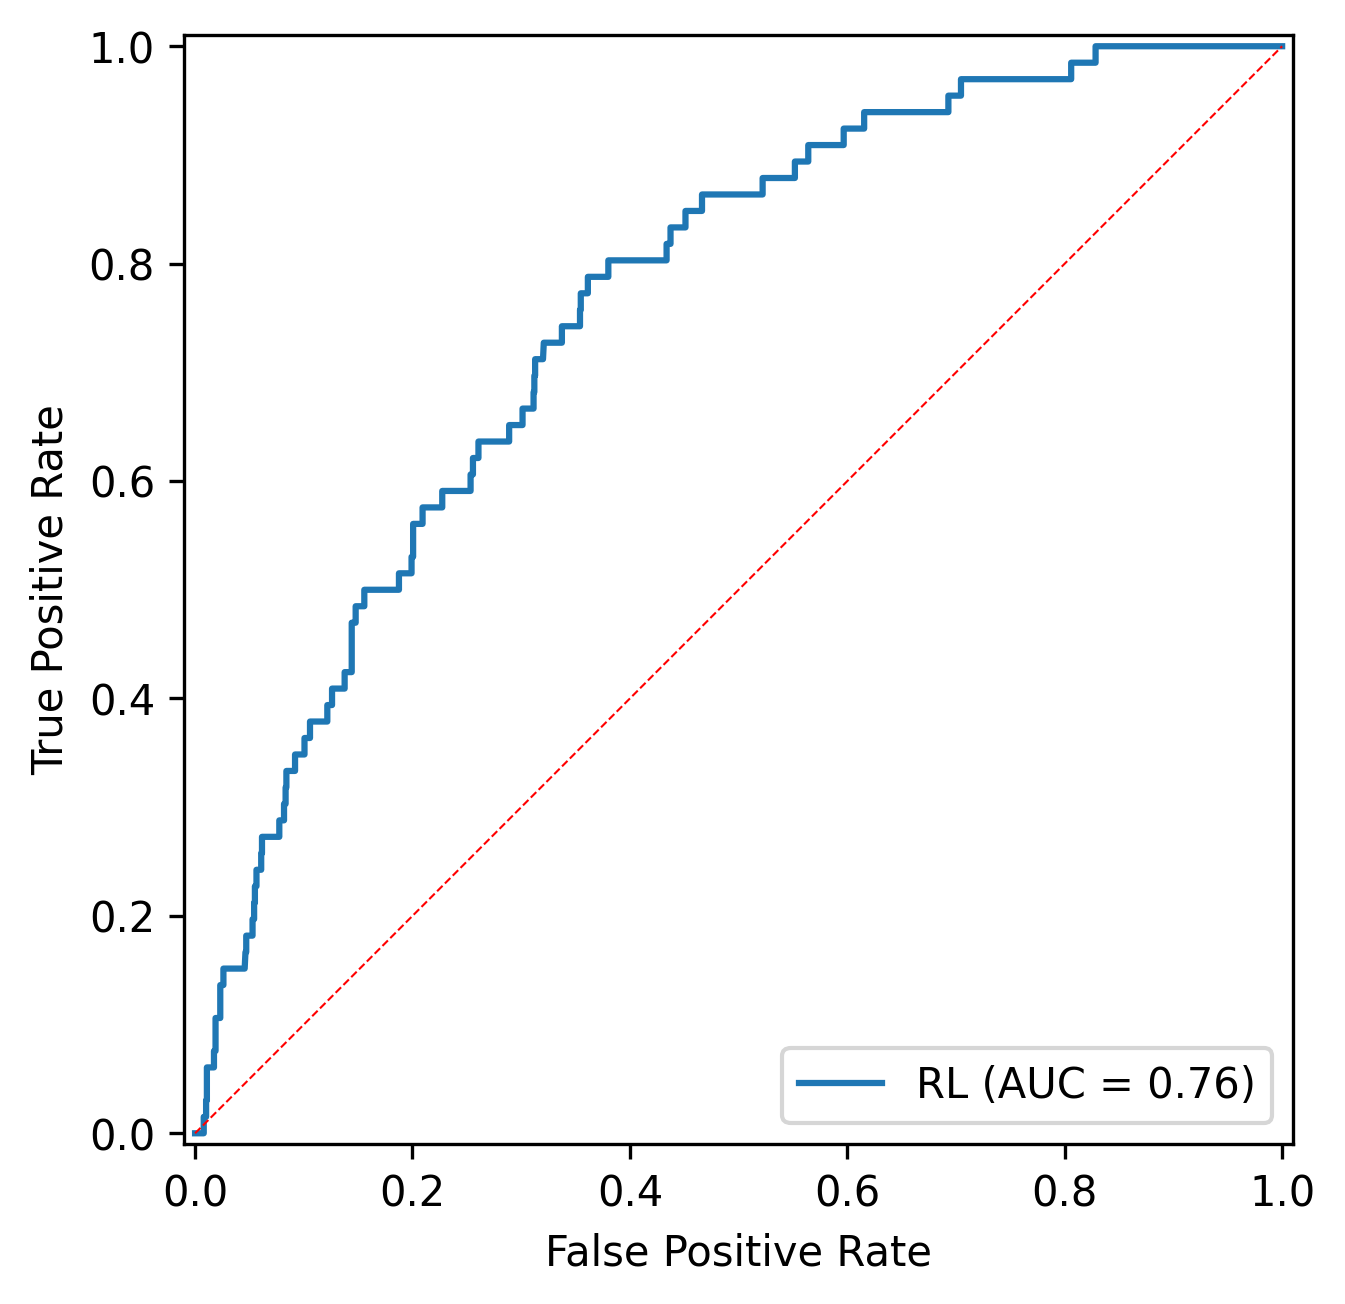
\includegraphics[width=0.3\linewidth]{reg-log-2004.png}
    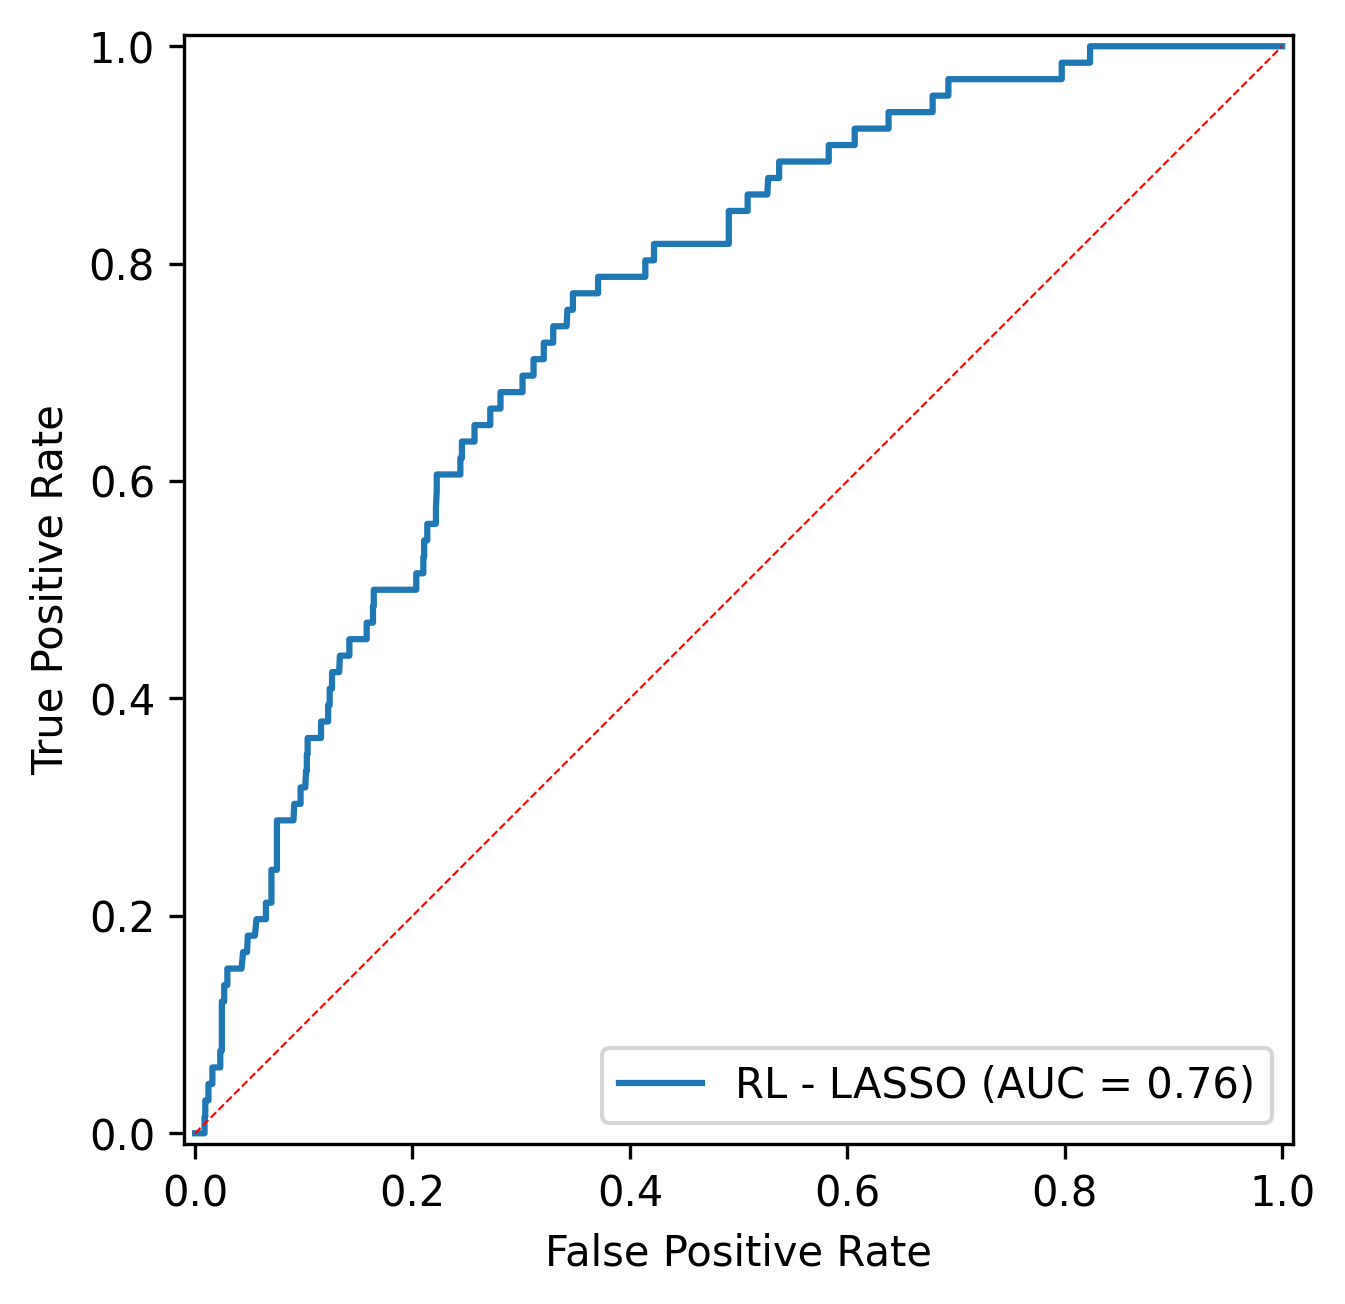
\includegraphics[width=0.3\linewidth]{lasso-2004.png}
    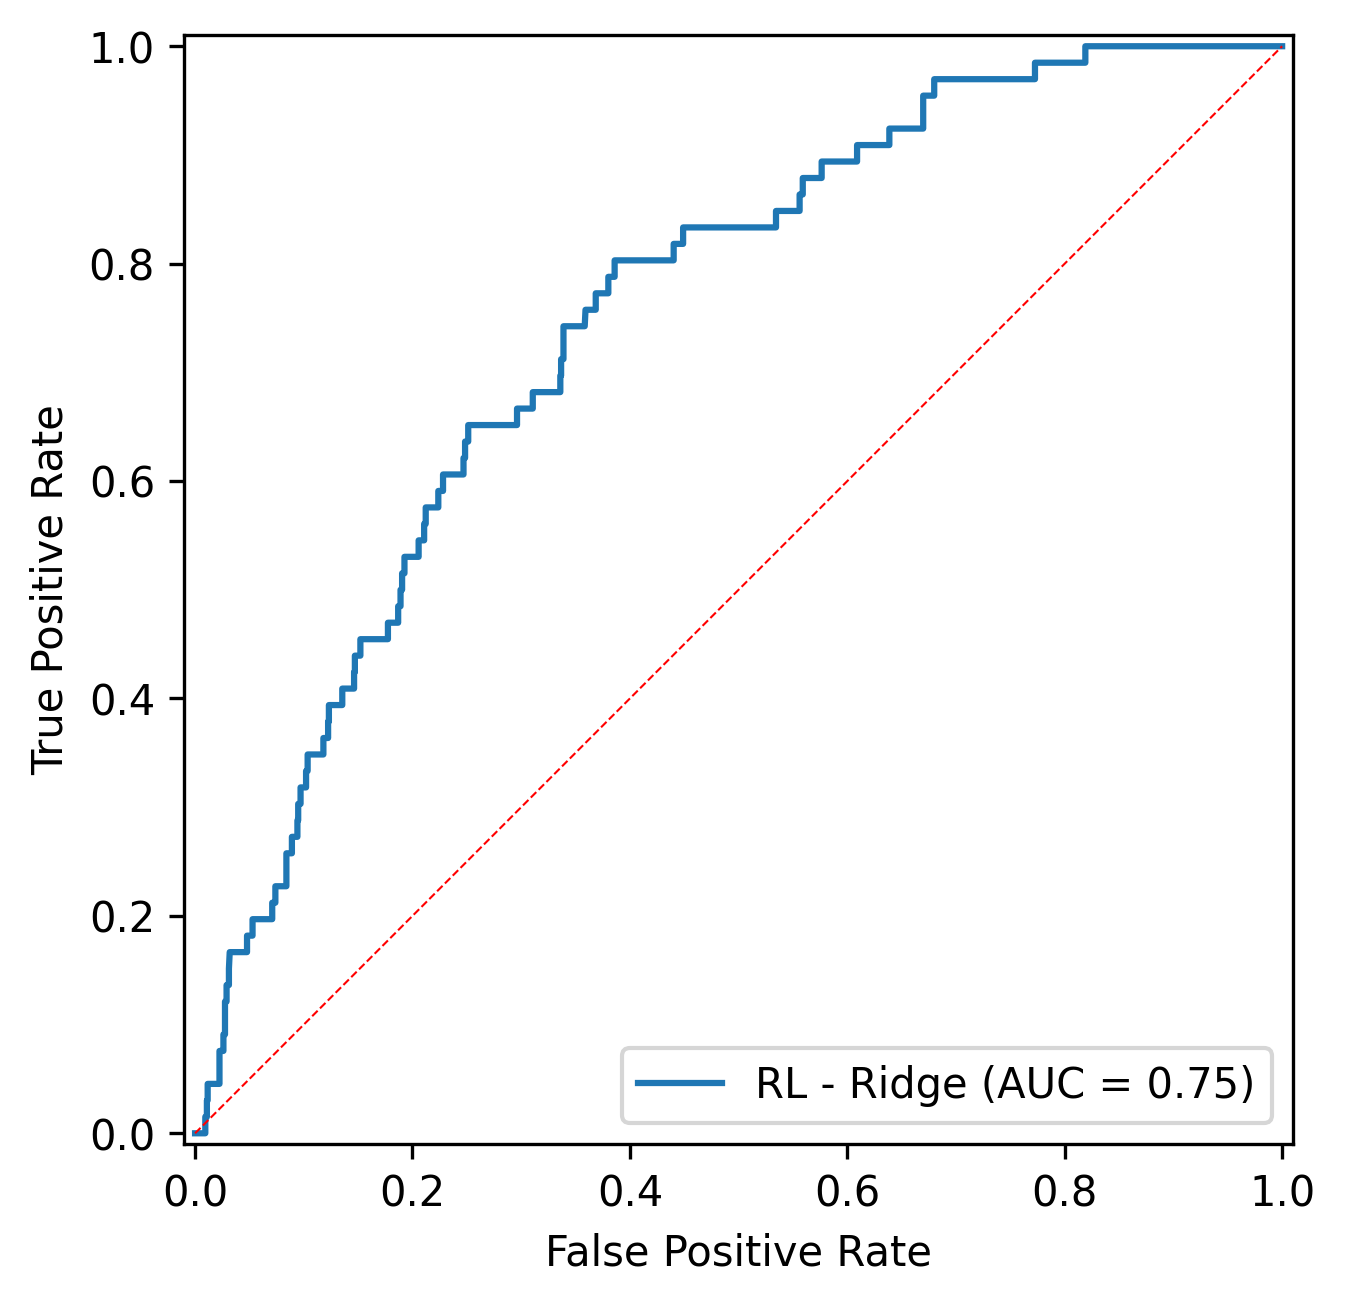
\includegraphics[width=0.3\linewidth]{ridge-2004.png}
\end{figure}

\begin{figure}[H]
    \centering
    \caption{Regresión Logística - 2024}
    \label{fig:roc2024}
    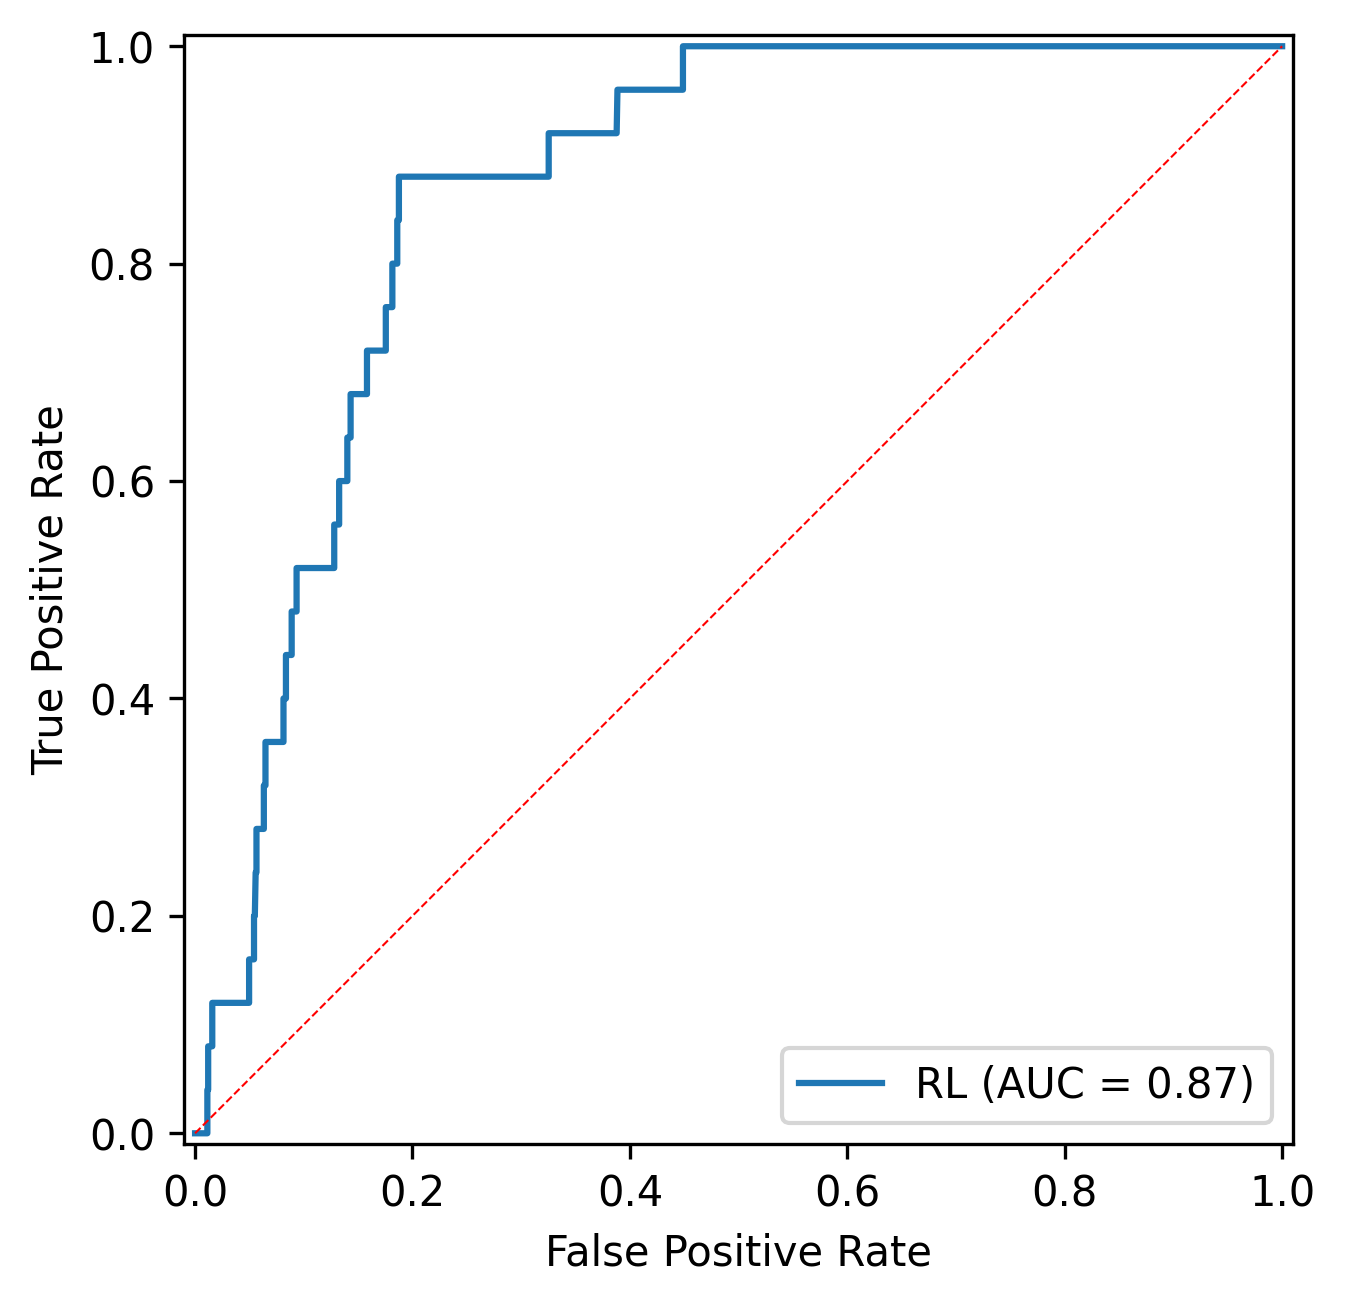
\includegraphics[width=0.3\linewidth]{reg-log-2024.png}
    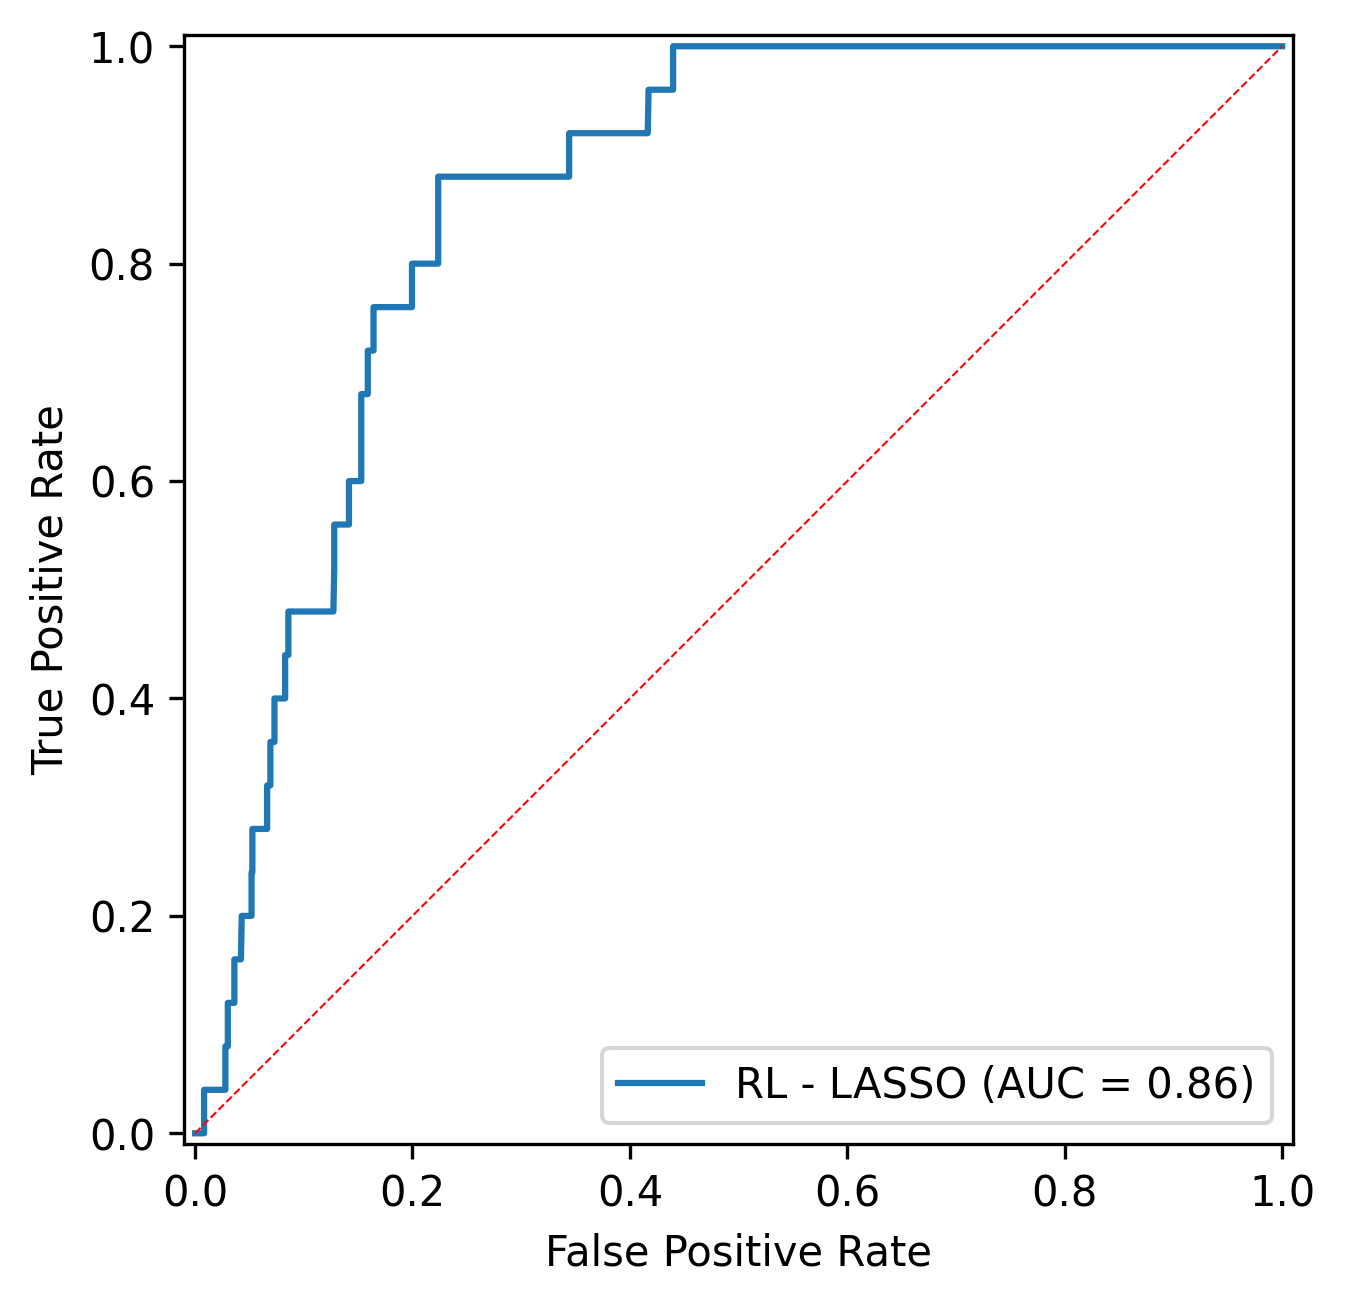
\includegraphics[width=0.3\linewidth]{lasso-2024.png}
    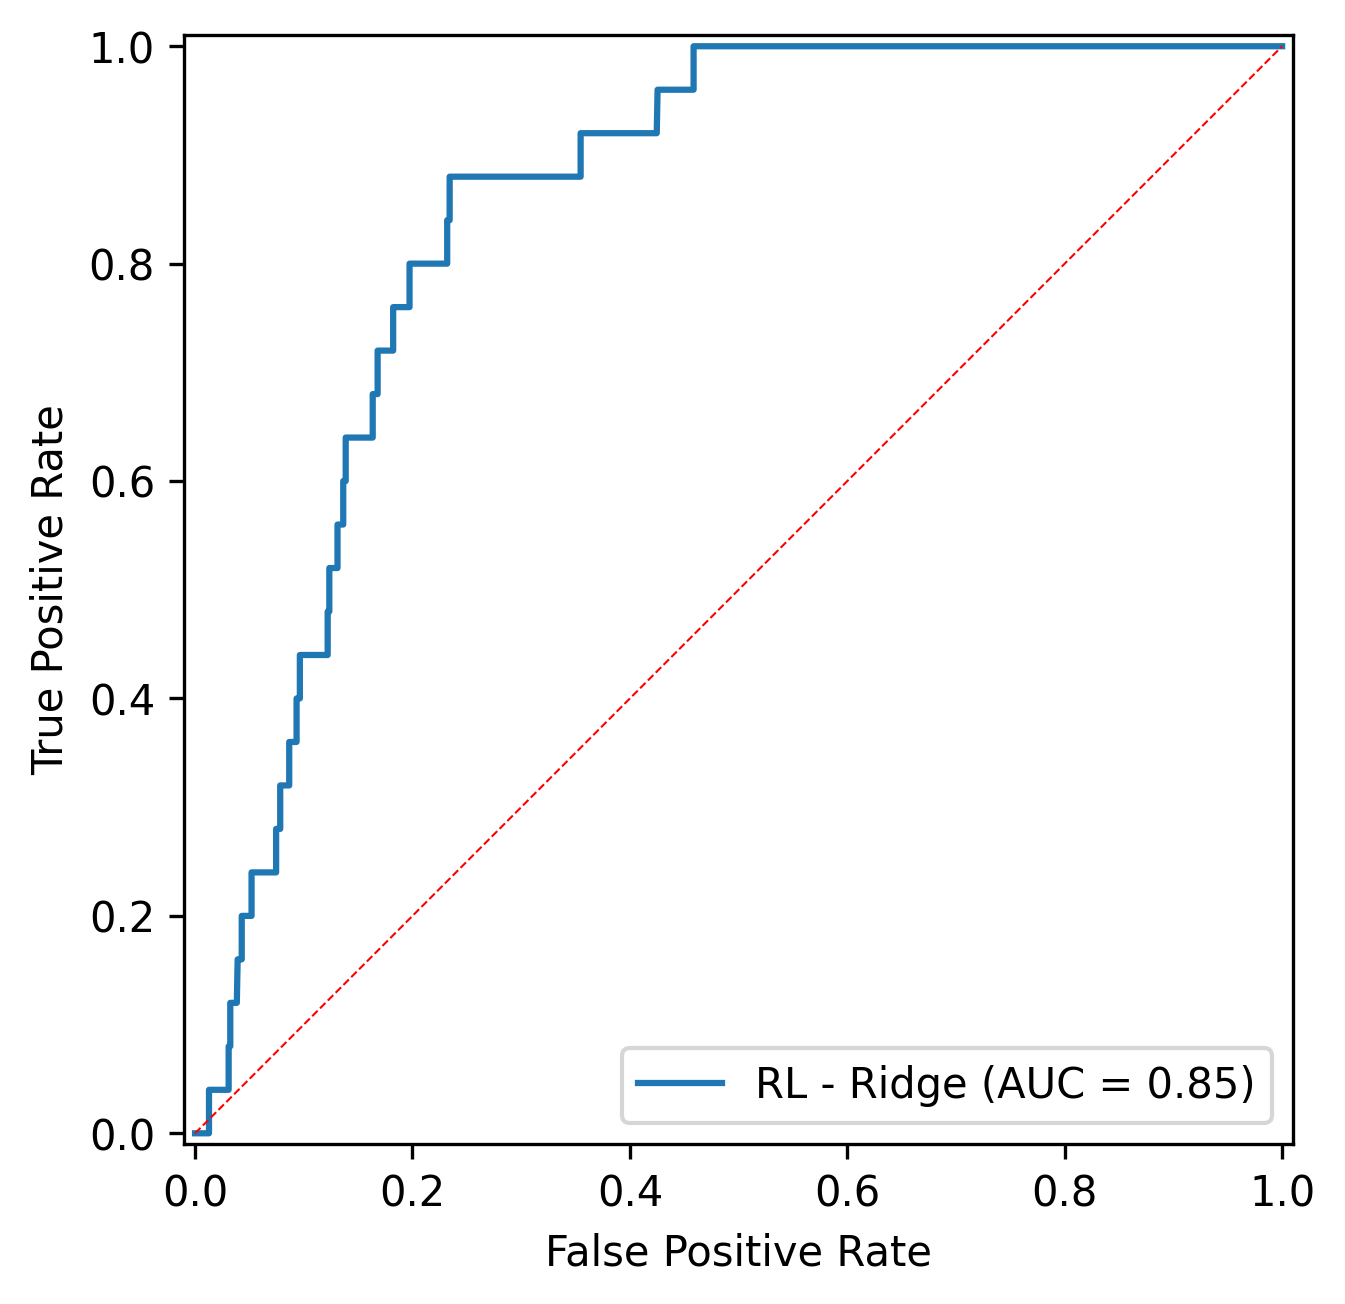
\includegraphics[width=0.3\linewidth]{ridge-2024.png}
\end{figure}

\subsection*{Ejercicio 4}

Al realizar un barrido de valores de \(\lambda\) en el rango \(10^n\) con \(n \in [-5, 5]\), utilizando validación cruzada de 10 folds, se obtuvieron resultados consistentes para los modelos de regresión logística con penalización LASSO y Ridge en los años 2004 y 2024. Para LASSO, el valor óptimo de \(\lambda\) fue \(10^{-4.0}\) tanto en 2004 como en 2024. En el caso de Ridge, el \(\lambda\) óptimo fue \(10^{1.0}\) en ambos años. Esto indica que LASSO funcionó mejor con una regularización débil (valores pequeños de \(\lambda\)), mientras que Ridge logró su mejor desempeño con una penalización más fuerte.

Las Figuras~\ref{fig:mse2004} y~\ref{fig:mse2024} muestran un gráfico de puntos conectados con el promedio del error cuadrático medio de testeo en los 10 folds para cada valor de \(\lambda\), para los años 2004 y 2024, respectivamente. En 2004, el promedio del MSE para LASSO fue más bajo y estable en los valores bajos de \(\lambda\), y comenzó a incrementarse a partir de \(10^{-2}\), alcanzando un valor constante desde \(10^{1}\) en adelante. Para Ridge, el MSE mínimo se registró precisamente en \(10^{1}\), lo que coincide con el valor de \(\lambda\) seleccionado como óptimo. En 2024 se observó una tendencia similar: el MSE promedio para LASSO fue más bajo entre \(10^{-5}\) y \(10^{-3}\), y luego aumentó con valores más altos de \(\lambda\).

\begin{figure}[H]
    \centering
    \caption{Promedio MSE test - 2004}
    \label{fig:mse2004}
    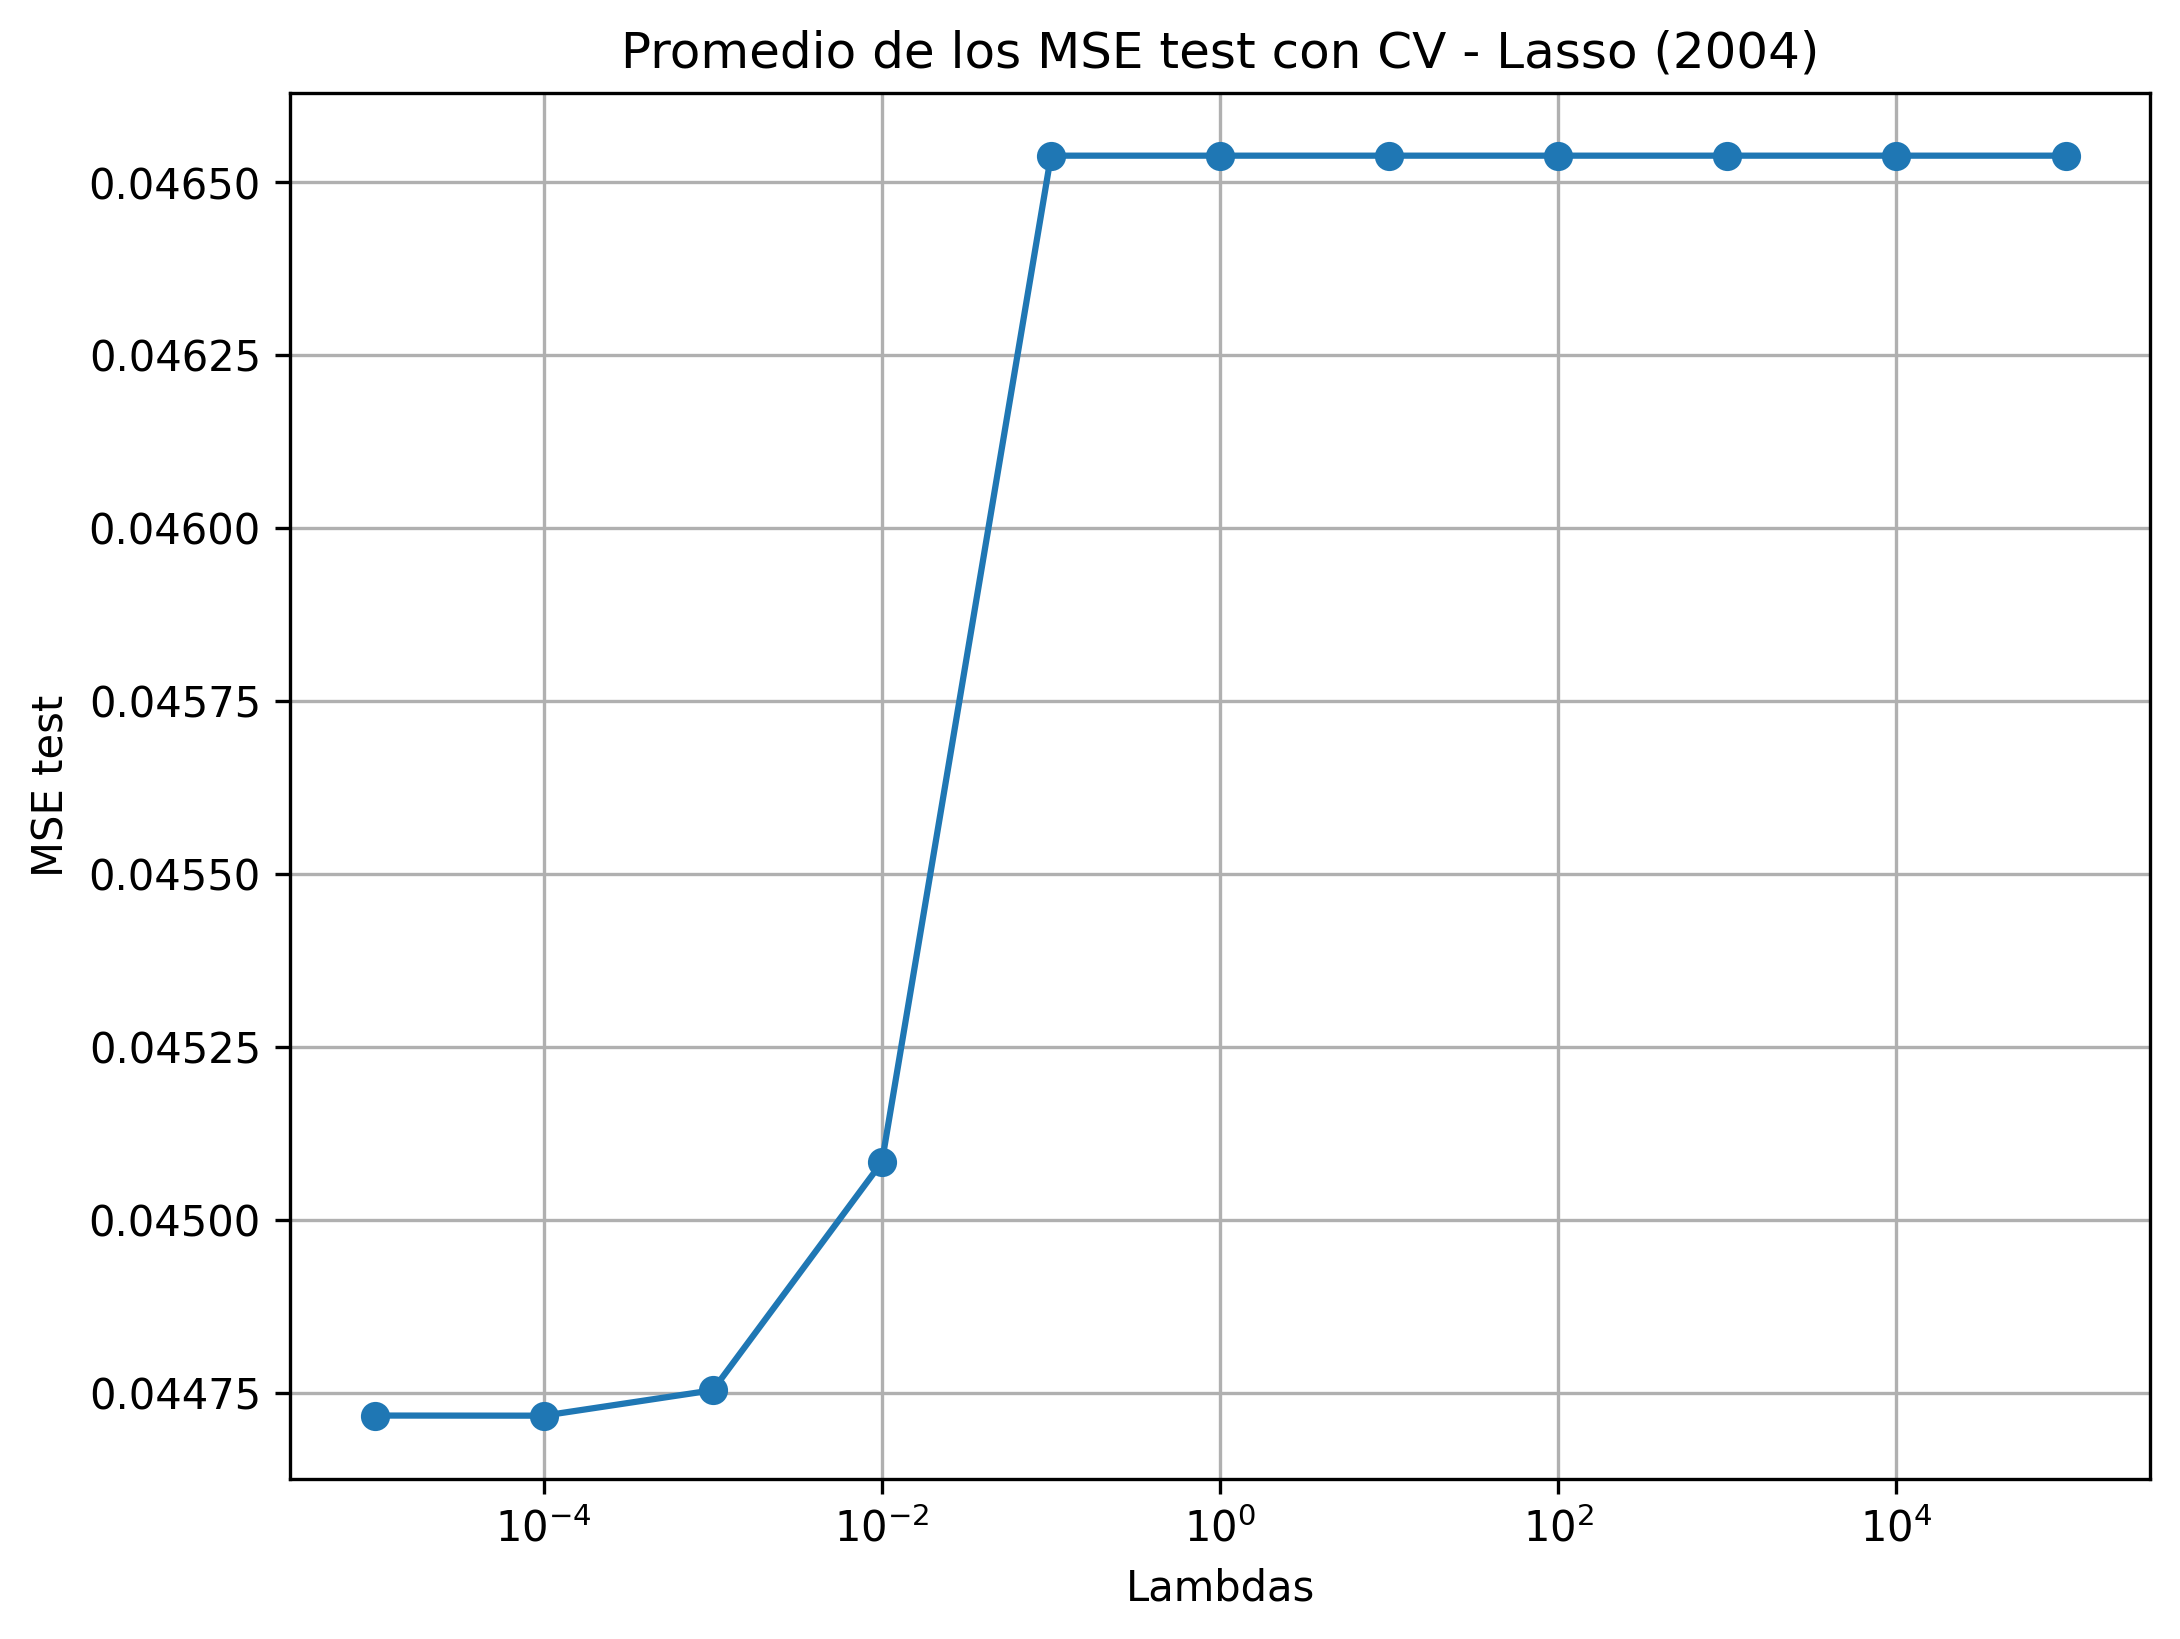
\includegraphics[width=0.4\linewidth]{mse-lasso-2004.png}
    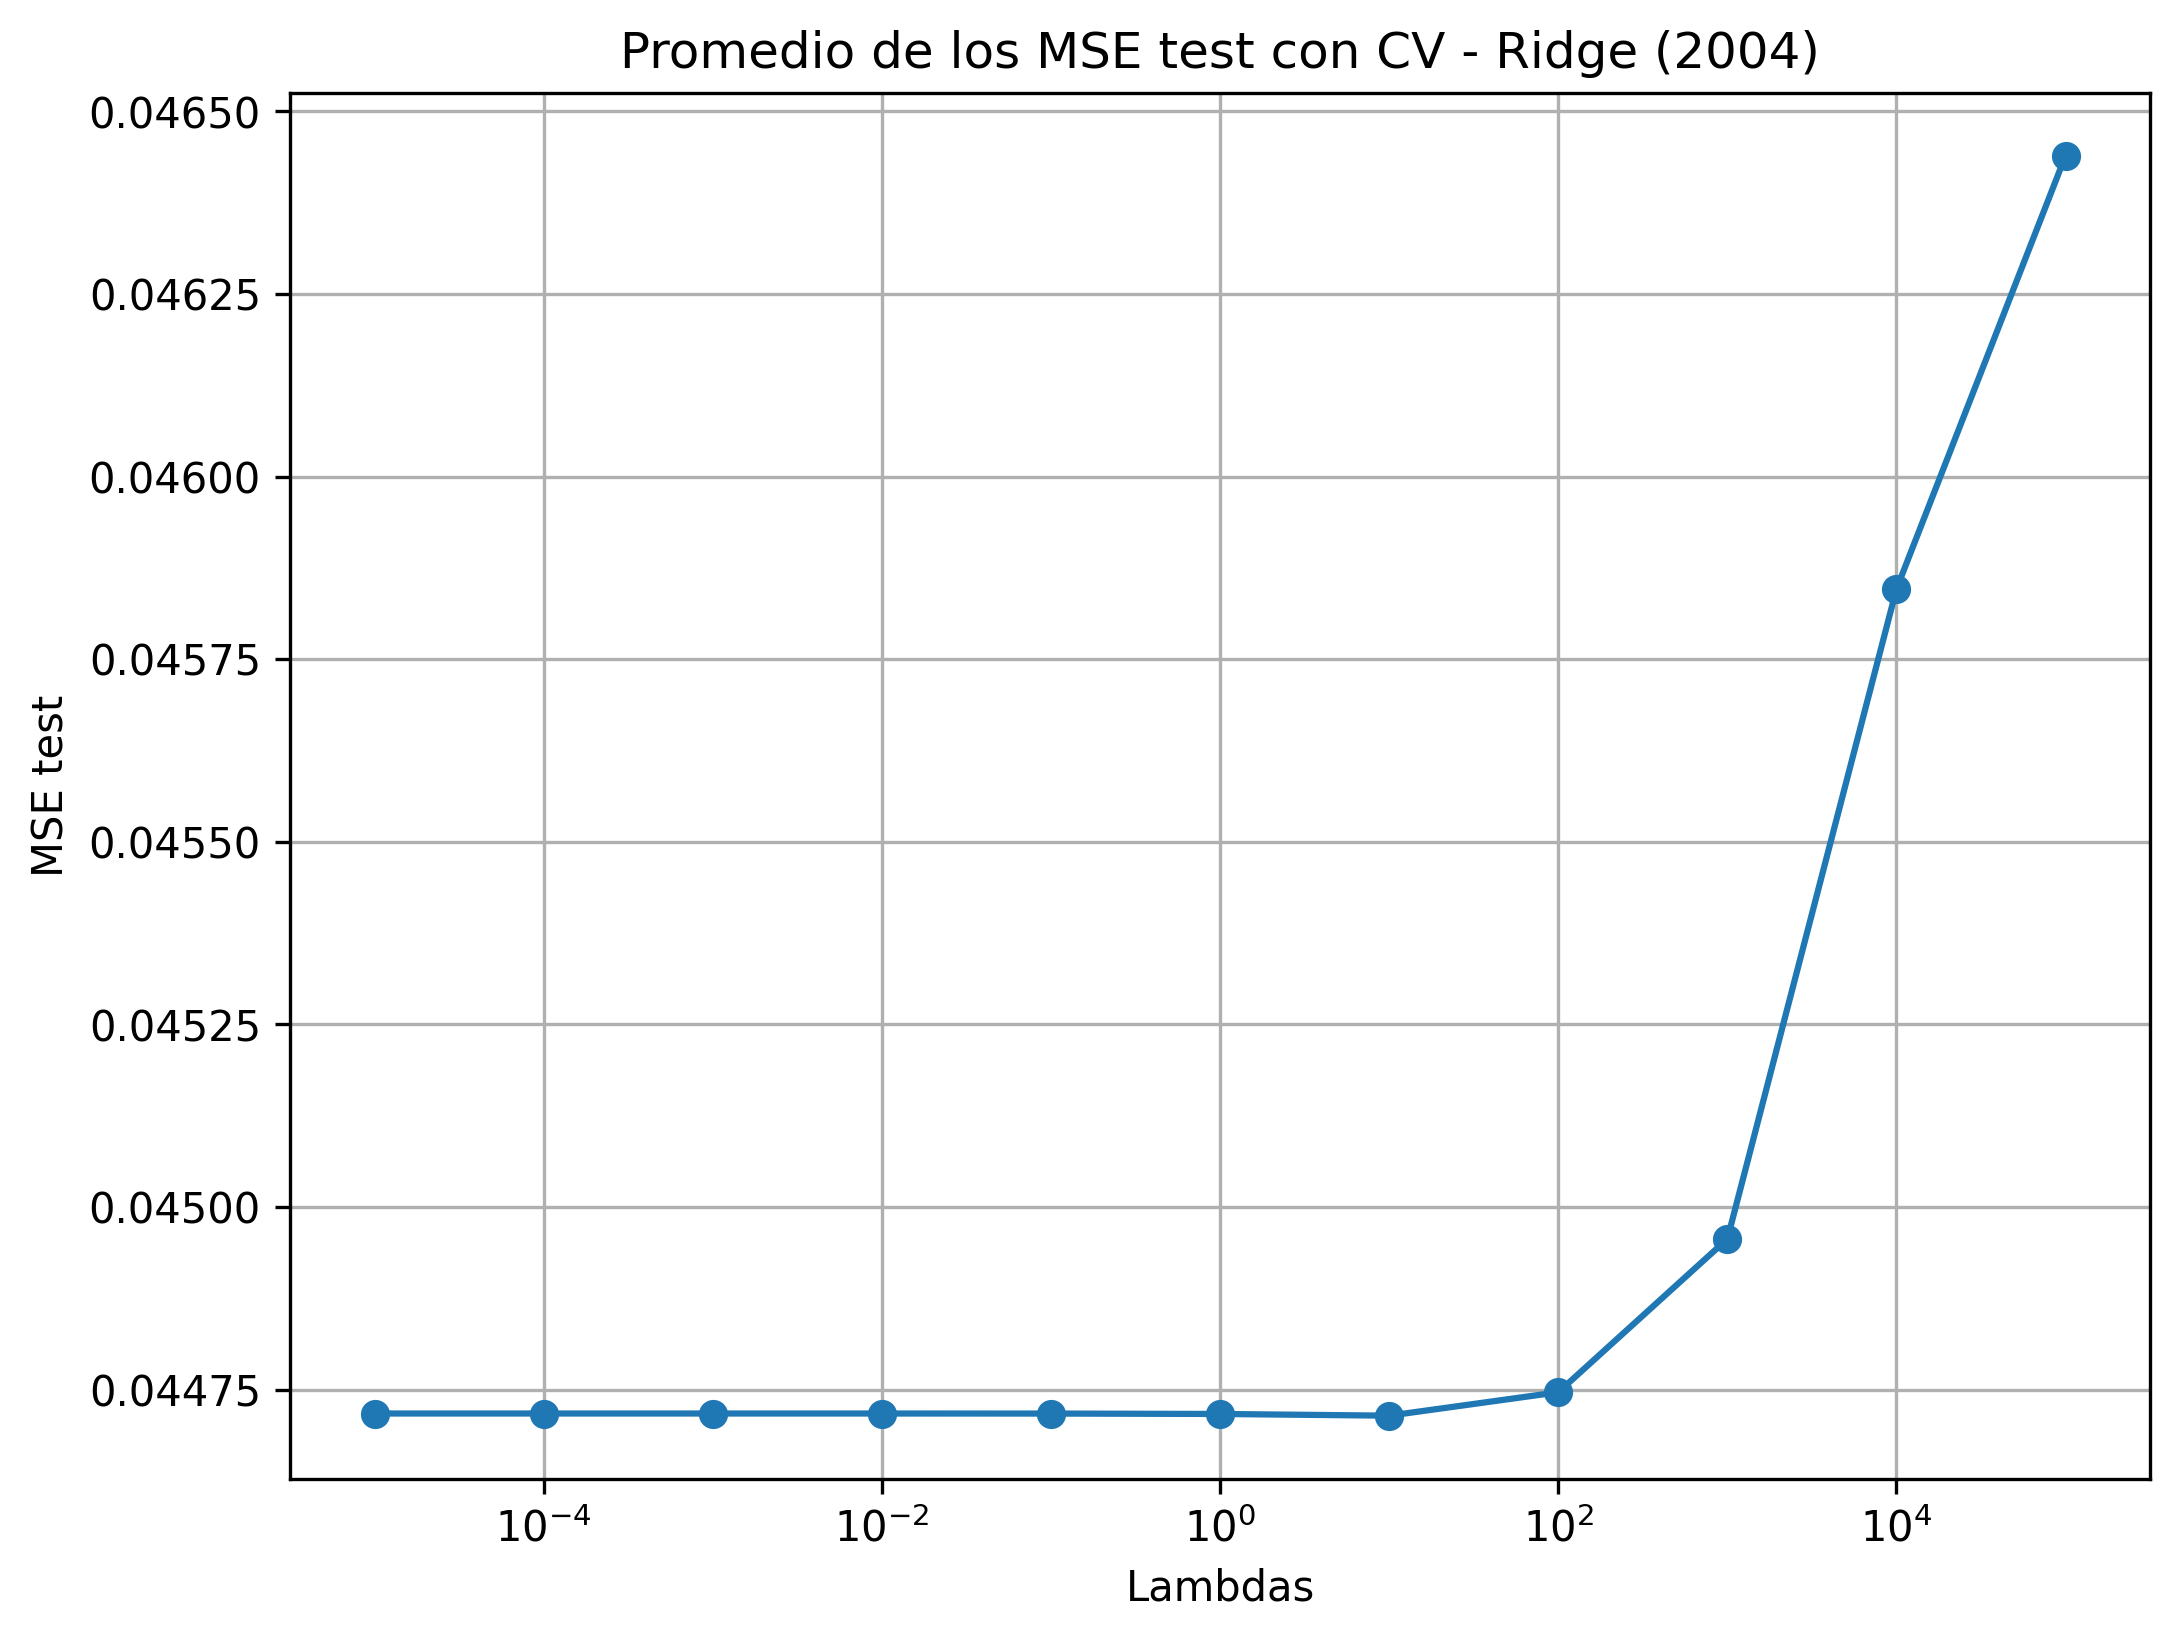
\includegraphics[width=0.4\linewidth]{mse-ridge-2004.png}
\end{figure}

\begin{figure}[H]
    \centering
    \caption{Promedio MSE test - 2024}
    \label{fig:mse2024}
    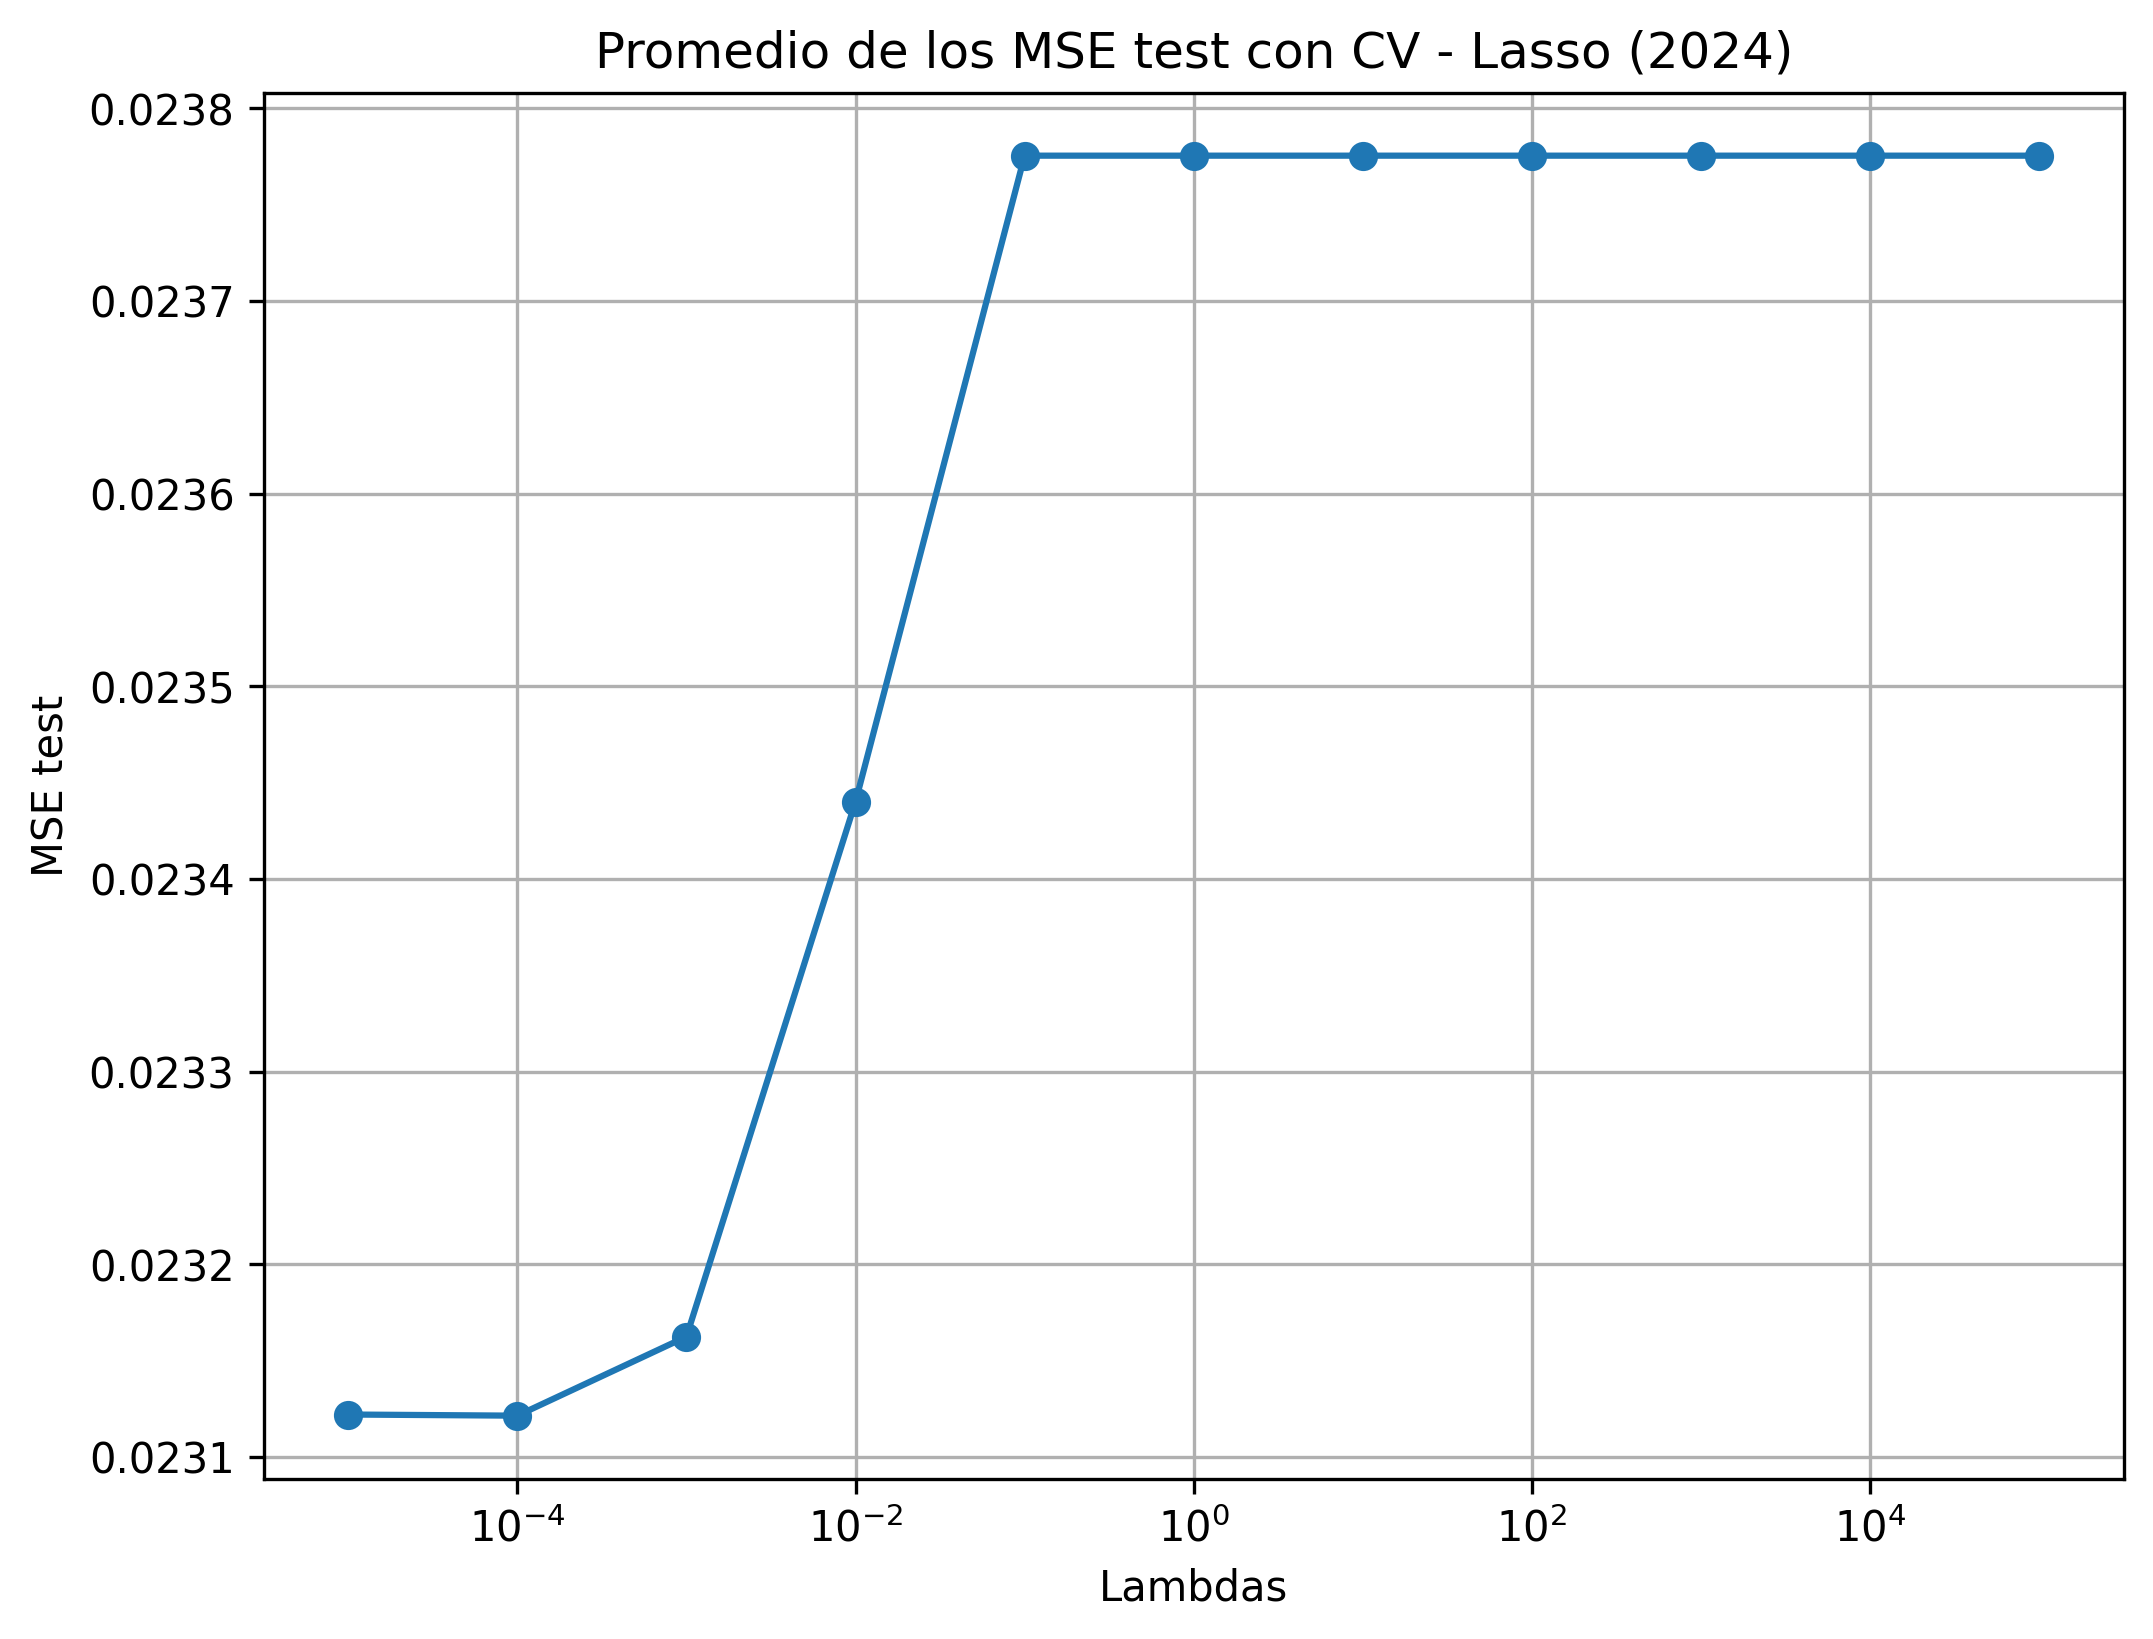
\includegraphics[width=0.4\linewidth]{mse-lasso-2024.png}
    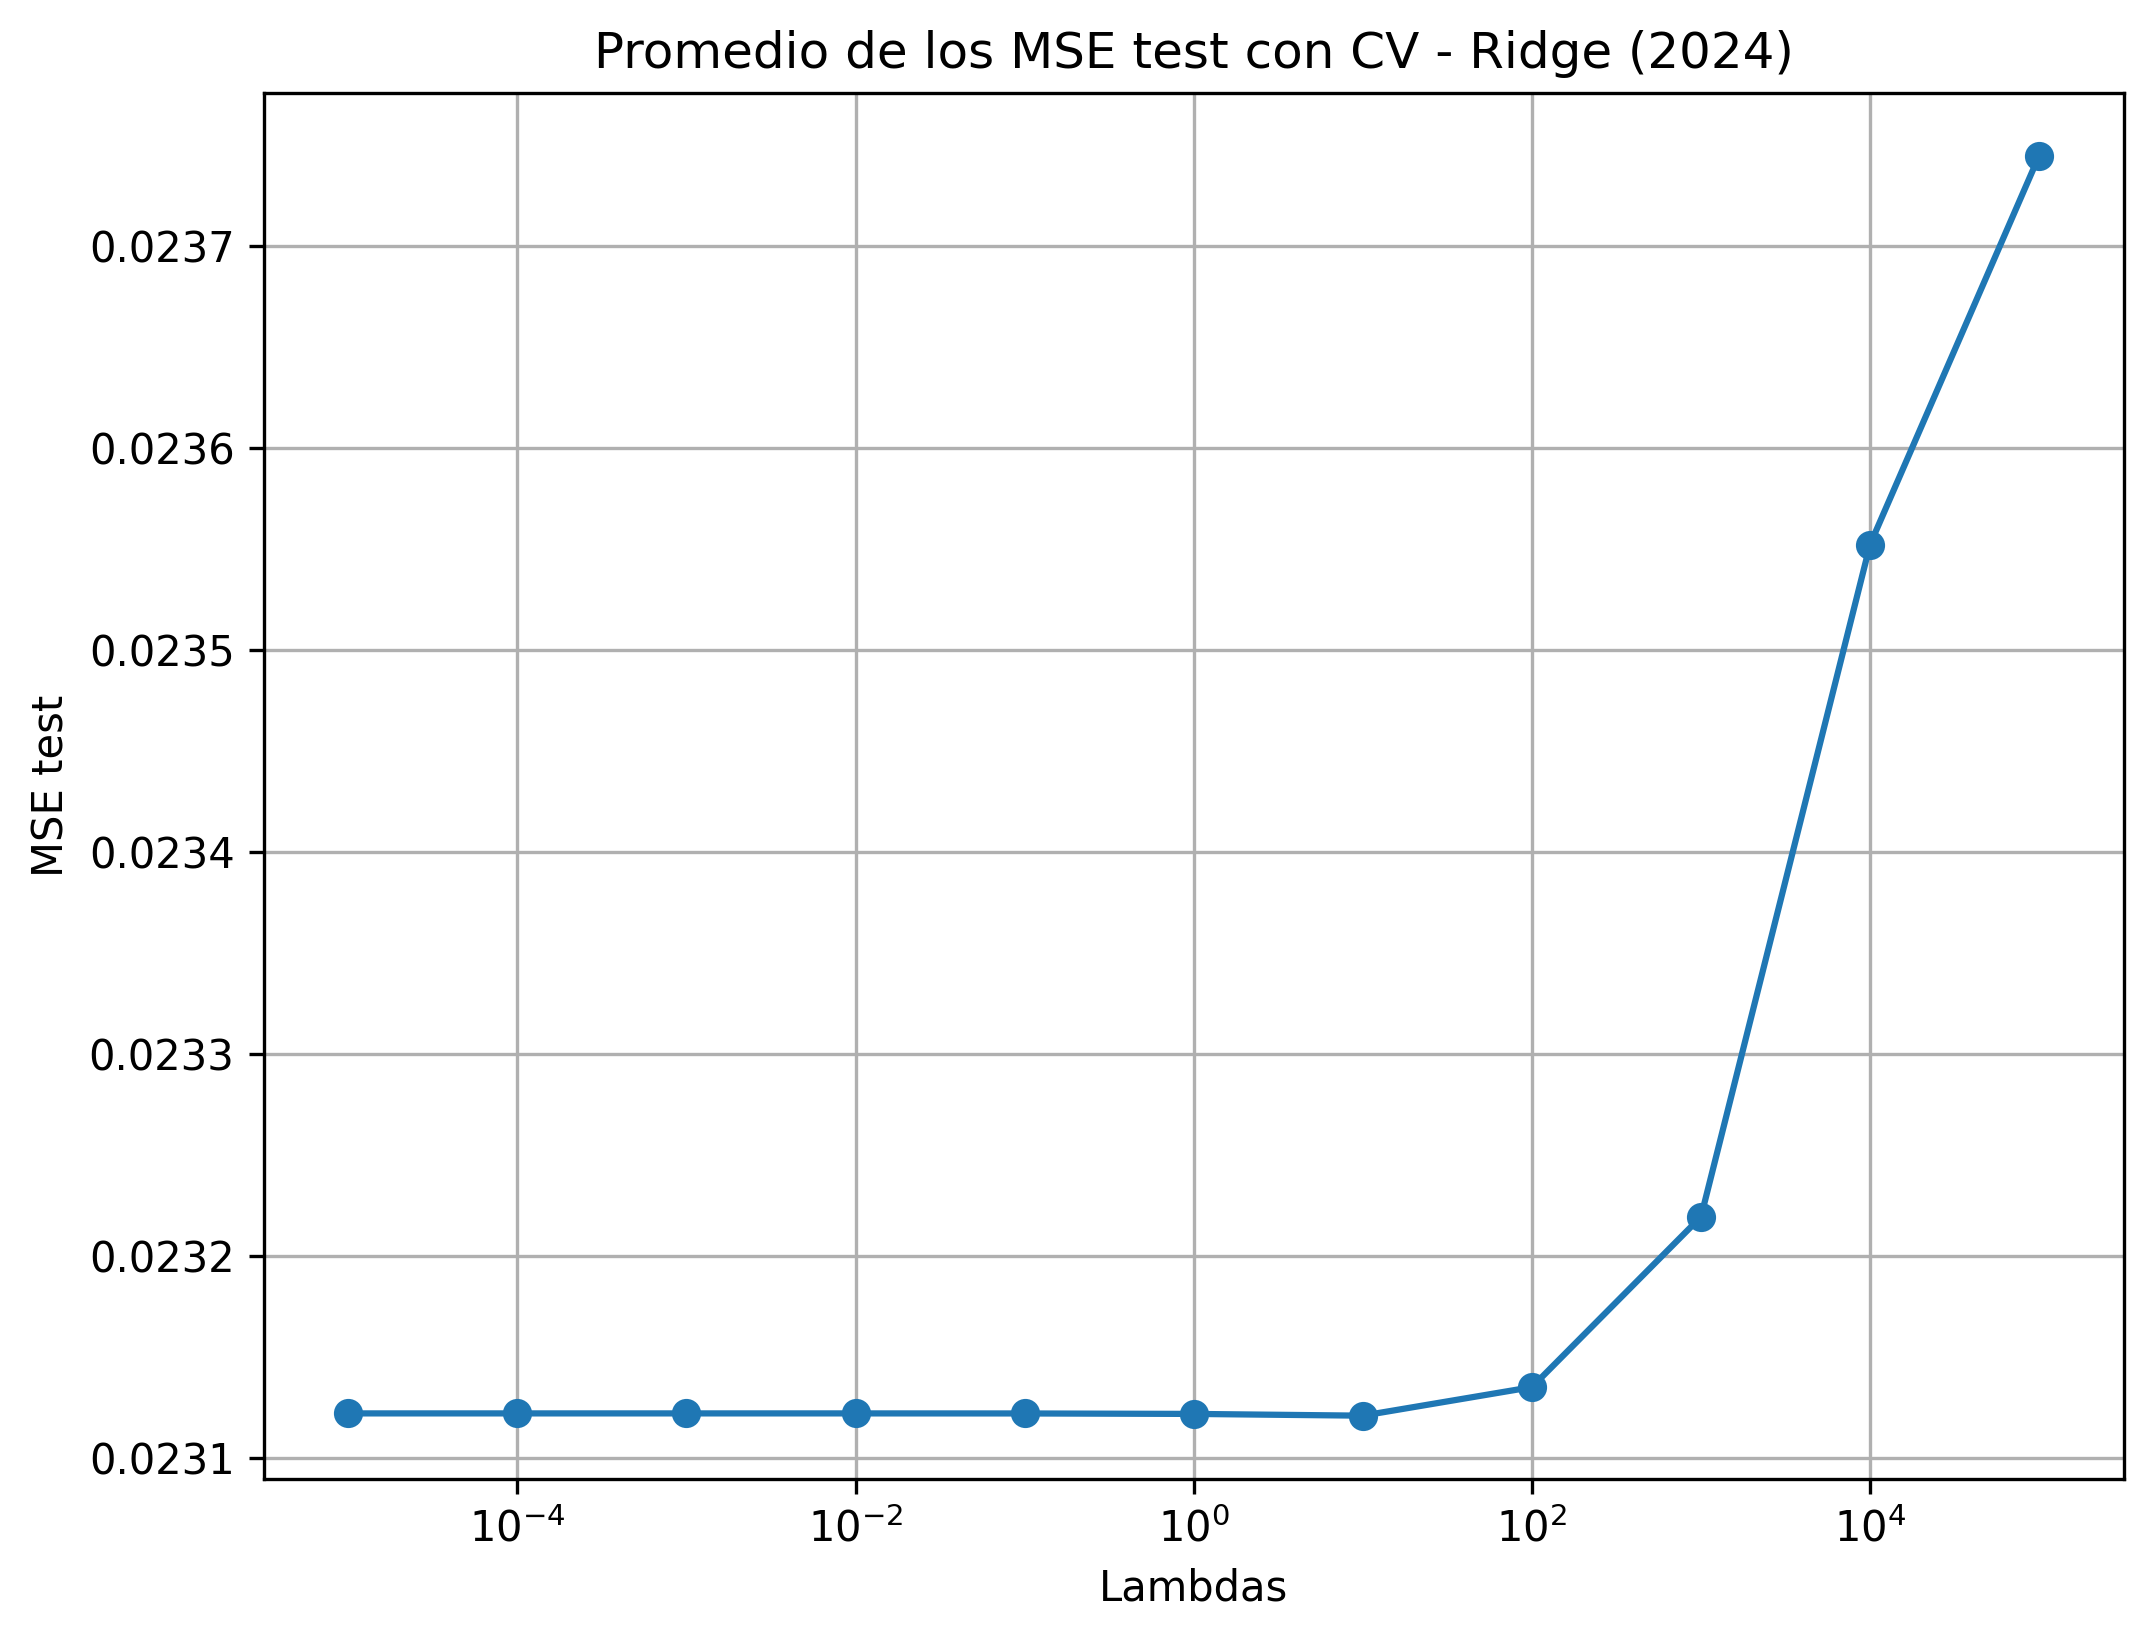
\includegraphics[width=0.4\linewidth]{mse-ridge-2024.png}
\end{figure}

En la Figura~\ref{fig:descartes}, vemos la proporción promedio de variables descartadas (coeficientes igual a cero) de LASSO en función de \(\lambda\). En ambos años, para \(\lambda\) pequeños (\(10^{-5}\) a \(10^{-3}\)), LASSO mantuvo la mayoría de las variables activas, descartando solo entre el 9\% y el 33\%. A partir de \(\lambda = 10^{-2}\), la proporción de variables descartadas aumentó abruptamente, llegando al 100\% desde \(\lambda = 10^{0}\), lo que implica que el modelo eliminó por completo todas las variables explicativas.

\begin{figure}[H]
    \centering
    \caption{Variables descartadas en función de \(\lambda\)}
    \label{fig:descartes}
    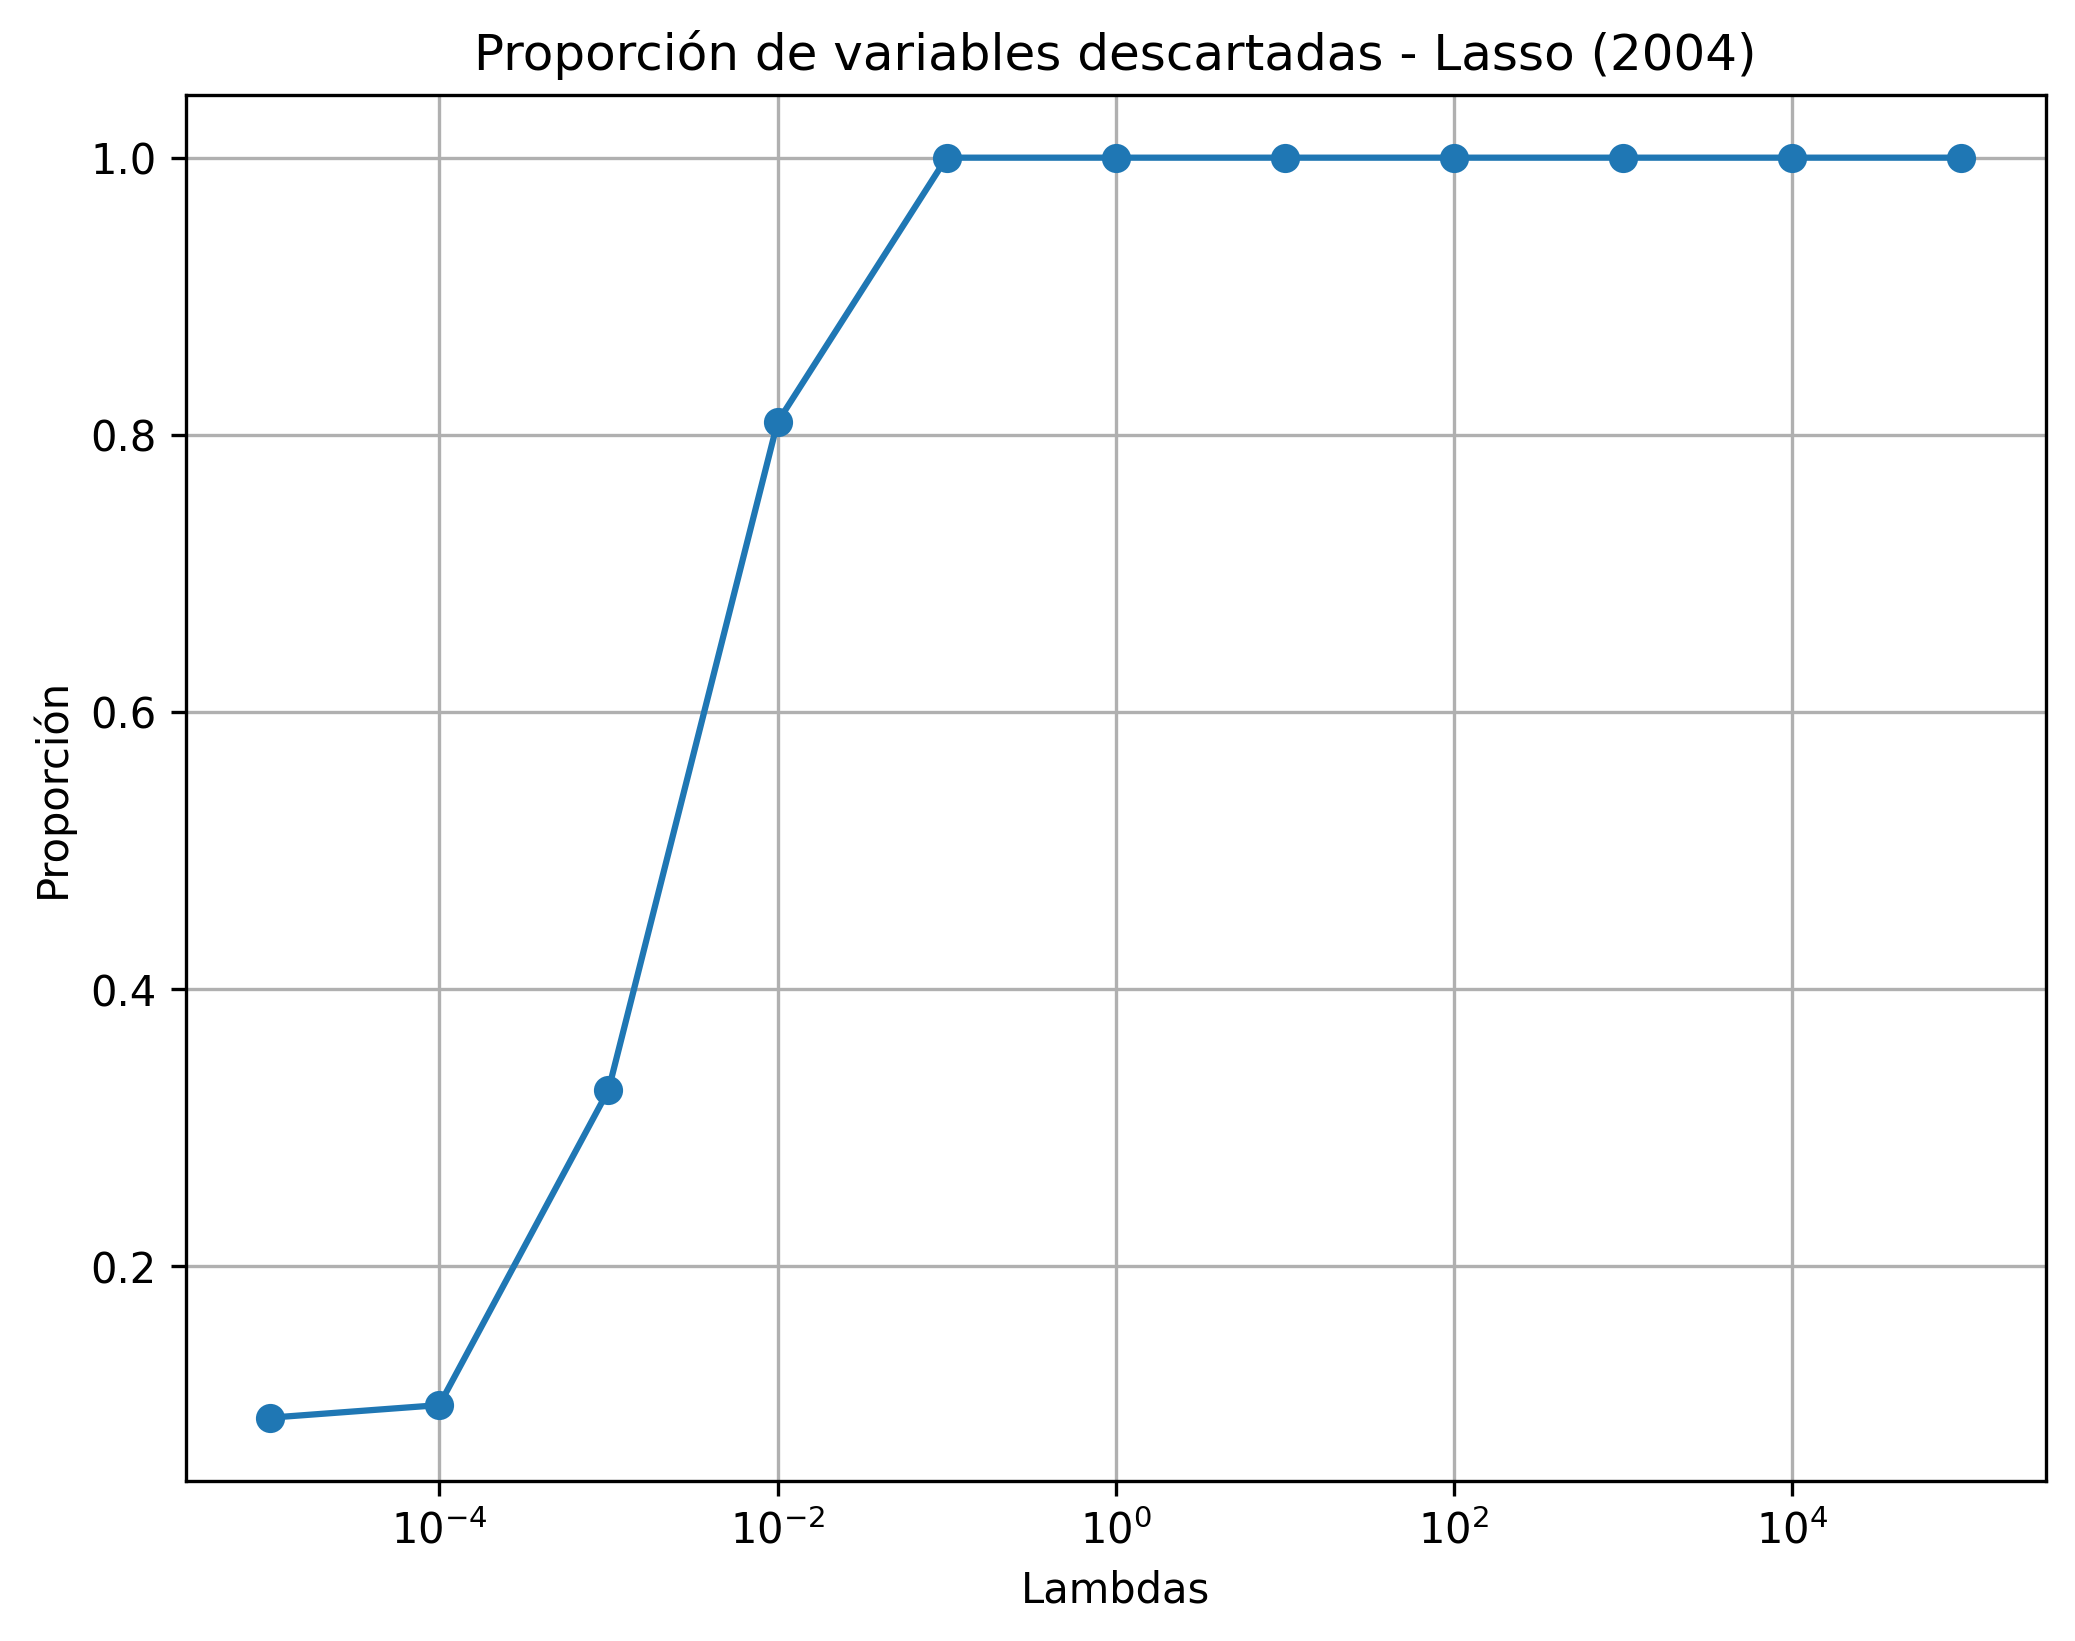
\includegraphics[width=0.4\linewidth]{descartes-lasso-2004.png}
    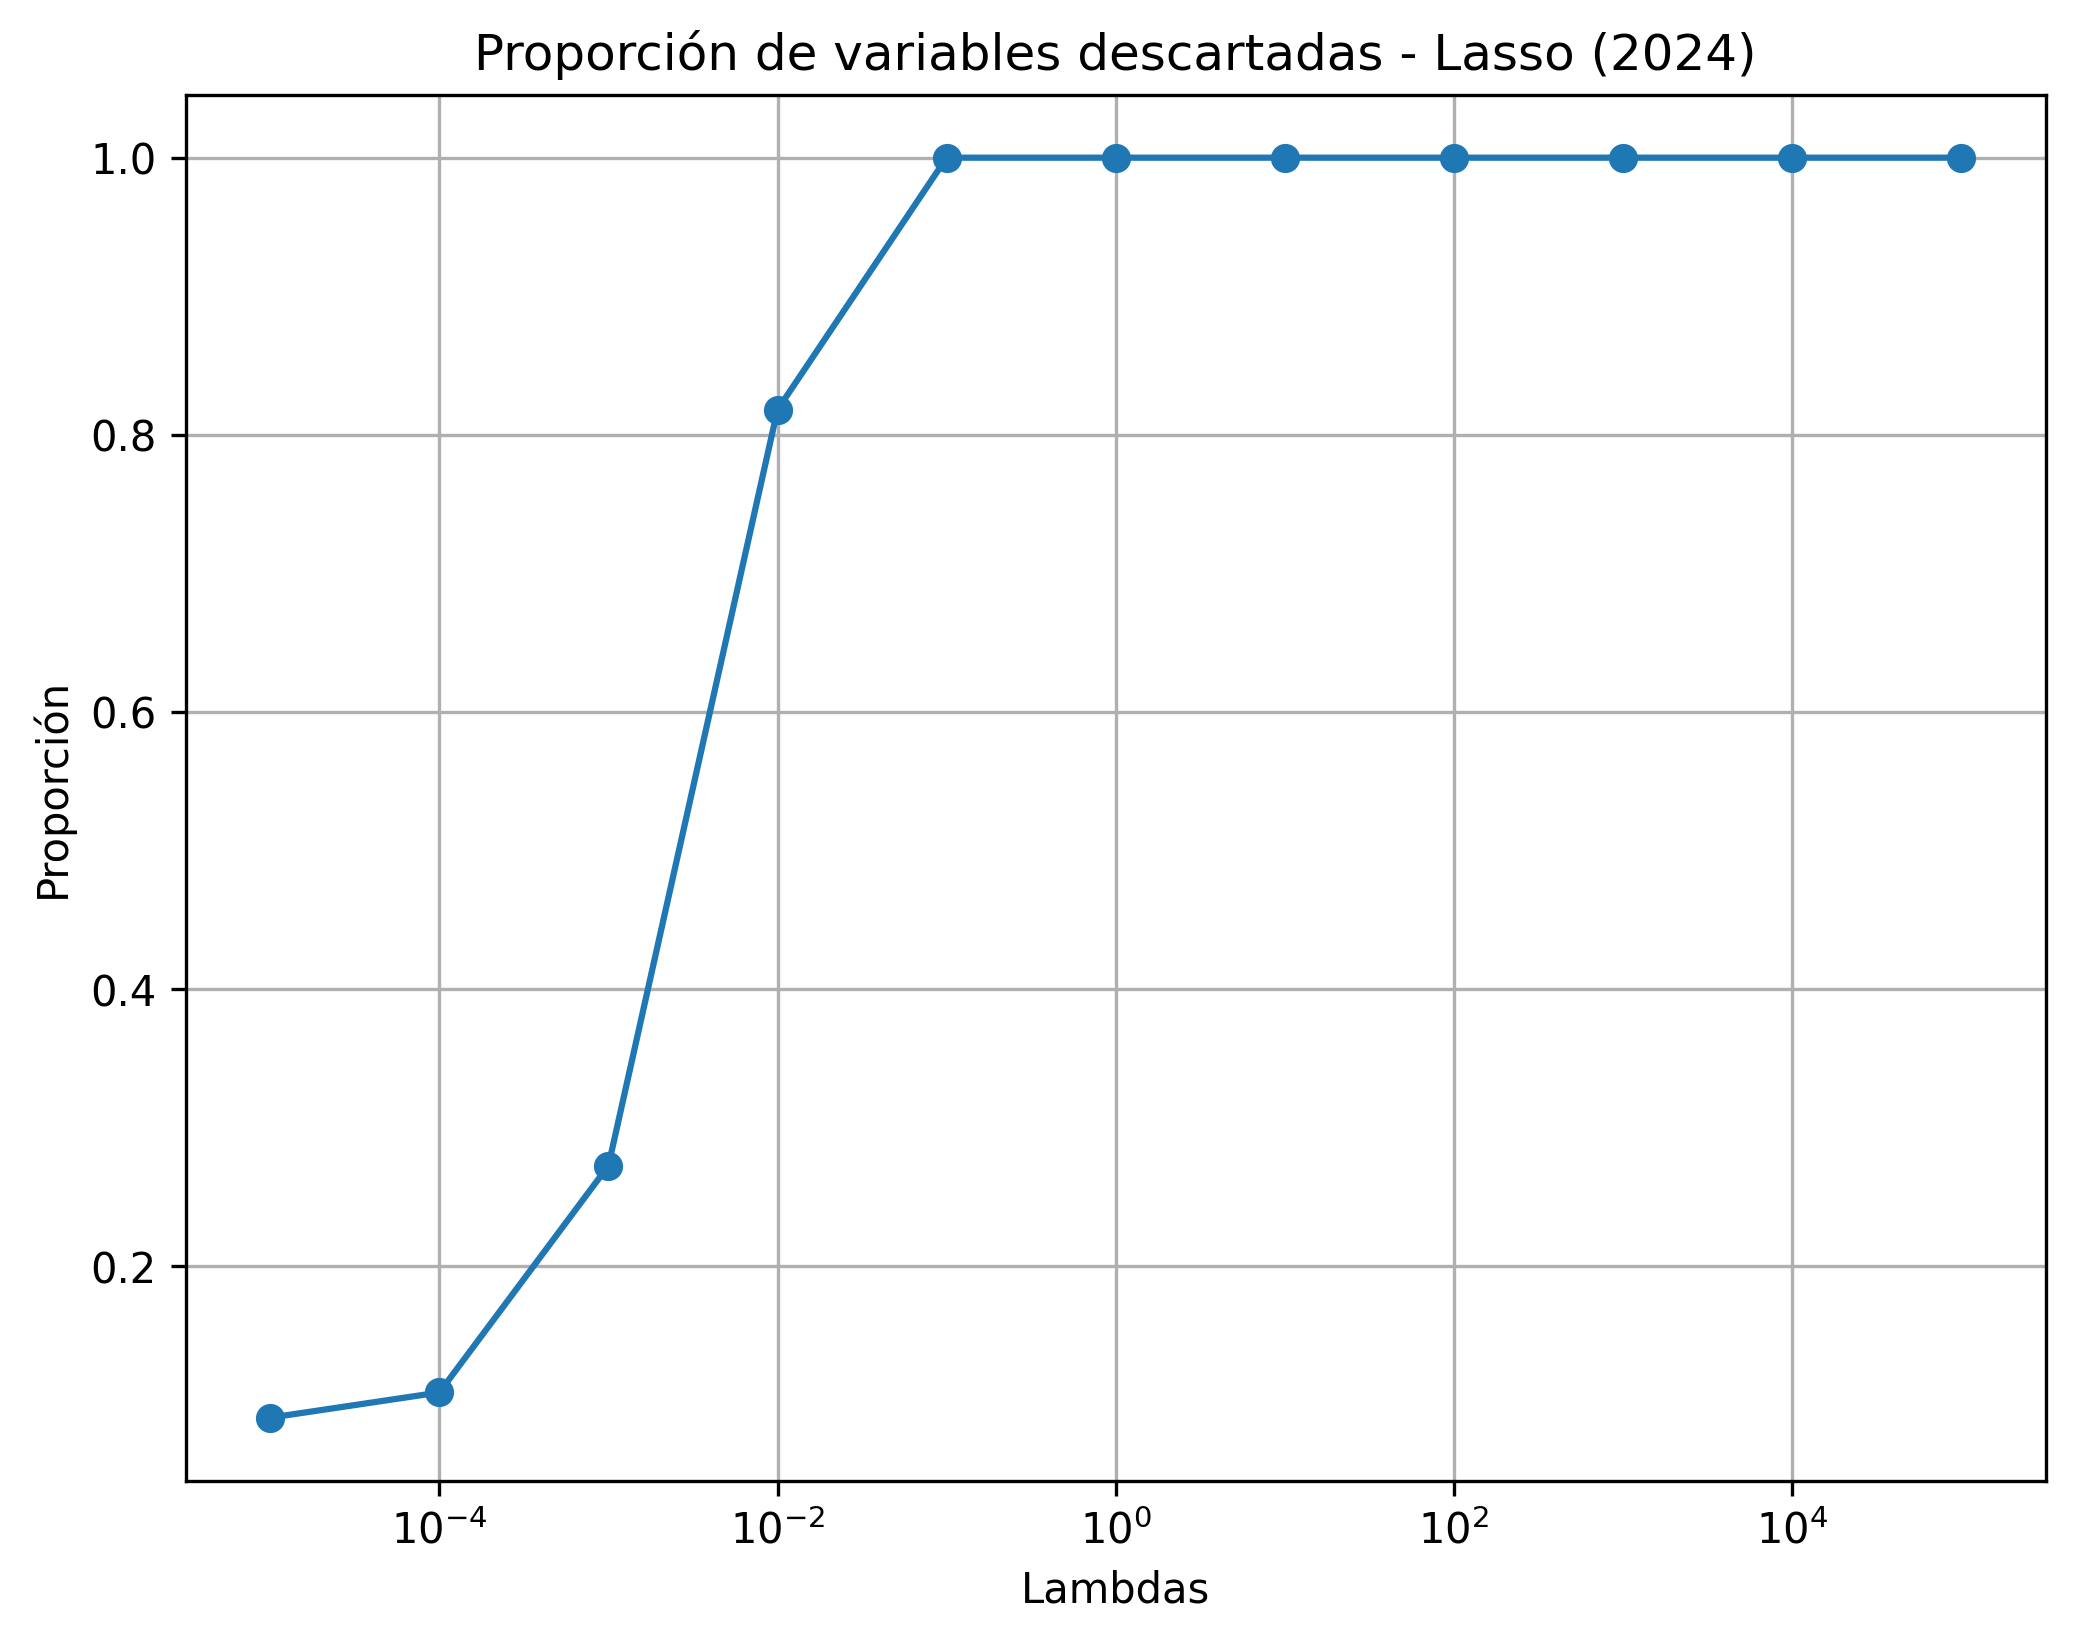
\includegraphics[width=0.4\linewidth]{descartes-lasso-2024.png}
\end{figure}

\subsection*{Ejercicio 5}

Para el valor óptimo de \(\lambda\) en LASSO, se observó que la única variable descartada fue la constante en ambos años, 2004 y 2024. Esto significa que ningún otro coeficiente asociado a las variables predictoras fue reducido a cero por la penalización, manteniendo activas todas las variables explicativas del modelo. Este resultado es coherente con lo que se esperaba, dado que el valor de \(\lambda\) seleccionado es bastante pequeño, lo que implica una penalización leve (y, por ende, que LASSO no elimine muchas variables).

\subsection*{Ejercicio 6}
% Lasso, 2004: El mean squared error de testeo es: 0.042126395120915684.
% Lasso, 2024: El mean squared error de testeo es: 0.017601039227447098
% Ridge, 2004: El mean squared error de testeo es: 0.04213340206837858
% Ridge, 2024: El mean squared error de testeo es: 0.0175981104374494

La métrica que se utiliza para determinar cuál fue el mejor método de regularización es el MSE de testeo. Encontramos que tanto para 2004 como para 2024, los errores son casi exactamente iguales entre LASSO y Ridge.

Para 2004, con LASSO se obtiene un MSE de testeo igual a 0.042126, mientras que con Ridge se llega a un valor de 0.042133. Podemos ver que, si bien ambos métodos son casi iguales, LASSO es ligeramente mejor.

Para 2024, se llega a un MSE de testeo de 0.01760 con LASSO y 0.01759 con Ridge. De nuevo, si bien son prácticamente iguales, hay una ligera ventaja con Ridge.

En términos generales, vemos que se obtiene un menor error en 2024 que en 2004. Esto se debe, probablemente, a que hay menos desocupados en la muestra de 2024. De nuevo, no es un indicador de que el método funcione mejor.

\section{Árboles}
\subsection*{Ejercicio 7}

La Figura~\ref{fig:arboles} muestra los dos árboles de decisión CART, seleccionando la profundidad máxima del árbol (\textit{max\_depth}) mediante validación cruzada con 10 folds, lo que resultó en un valor óptimo de 1 en ambos casos.

En 2004, el predictor principal fue la variable EDAD, con una división en menor o igual a 16.5 años. Este árbol mostró menores diferencias en la rama True (edad menor o igual a 16.5), es decir que allí había más no desocupados. Esto probablemente se debe a que la mayoría de ese grupo no entra en la categoría de económicamente activo, por lo que no pueden ser desocupados. Igualmente, en ambos casos la clase mayoritaria es no desocupado, así que nunca predice desocupado.

En 2024, el predictor utilizado fue la variable OBRA\_SOCIAL, que vale 0 si la persona depende total o parcialmente de servicios públicos de salud. Como se trata de una \textit{dummy}, la división en 0.5 indica que vale 0 en la rama True y 1 en la rama False. Se ve que el grupo que no depende del Estado para servicios de salud tiene menor cantidad de desocupados. Como en el otro árbol, nunca llega a predecir desocupado.

\begin{figure}[H]
    \centering
    \caption{Árboles de decisión (2004 vs 2024)}
    \label{fig:arboles}
    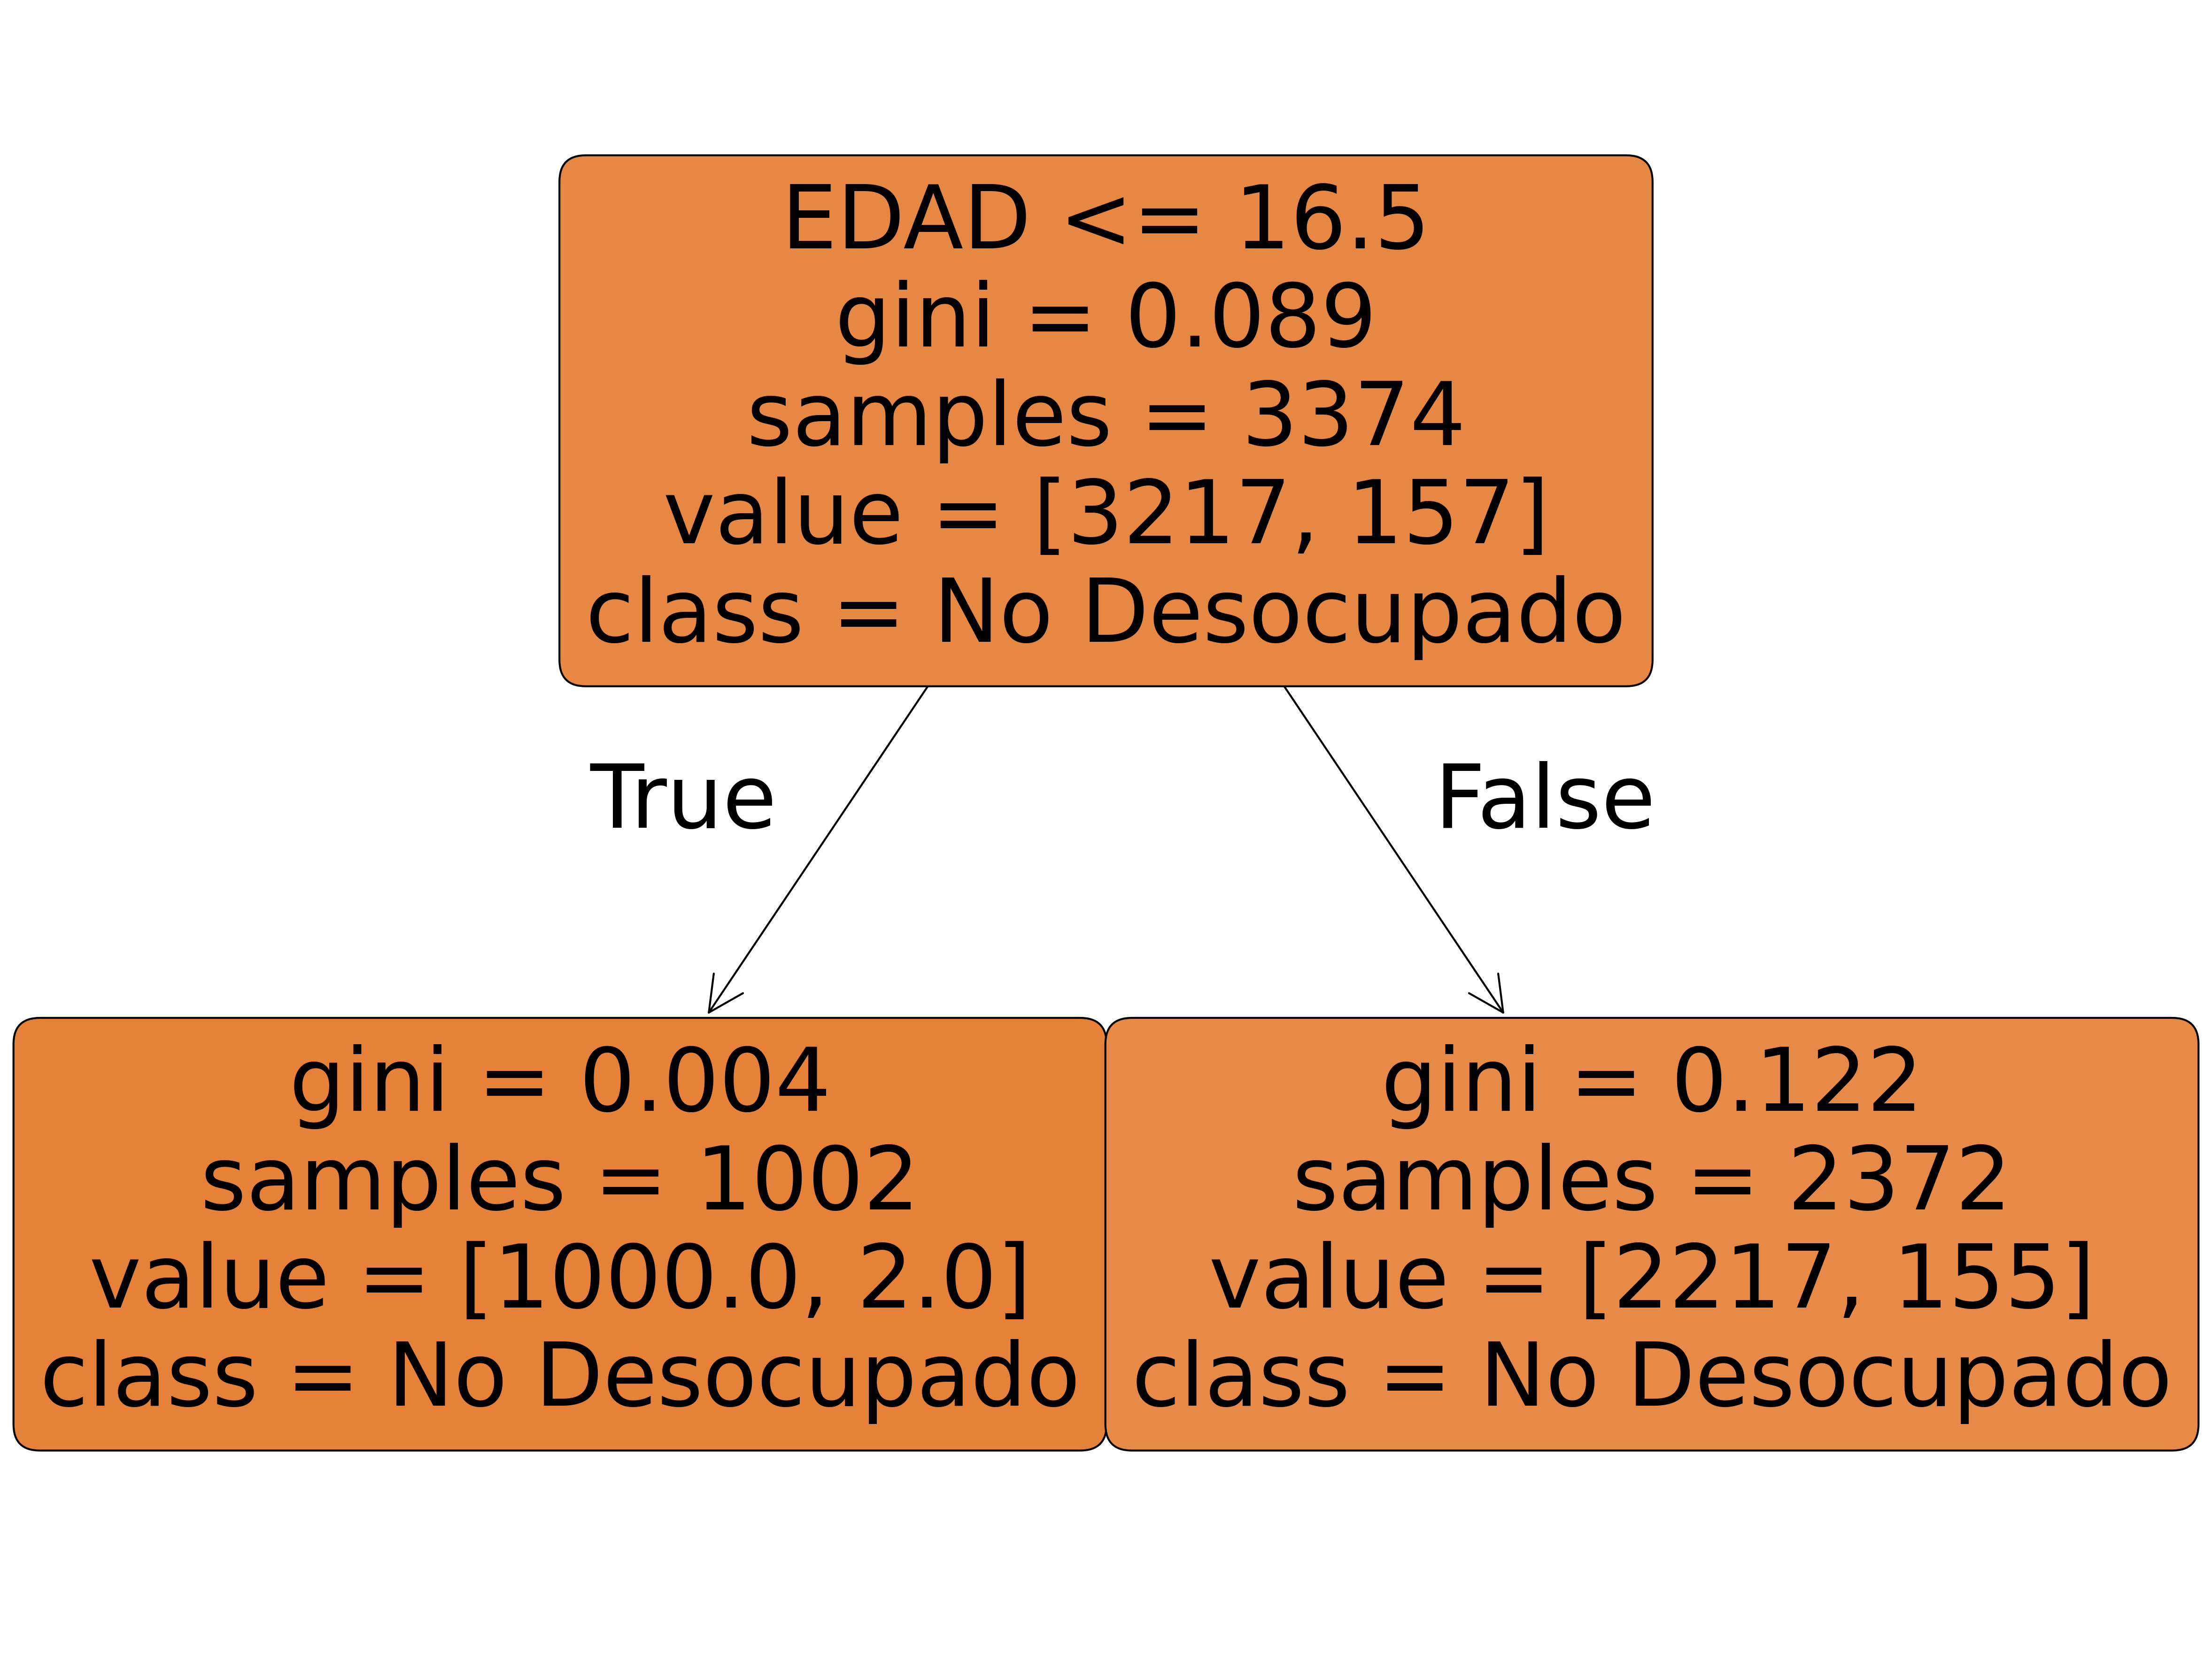
\includegraphics[width=0.45\linewidth]{arbol-2004.png}
    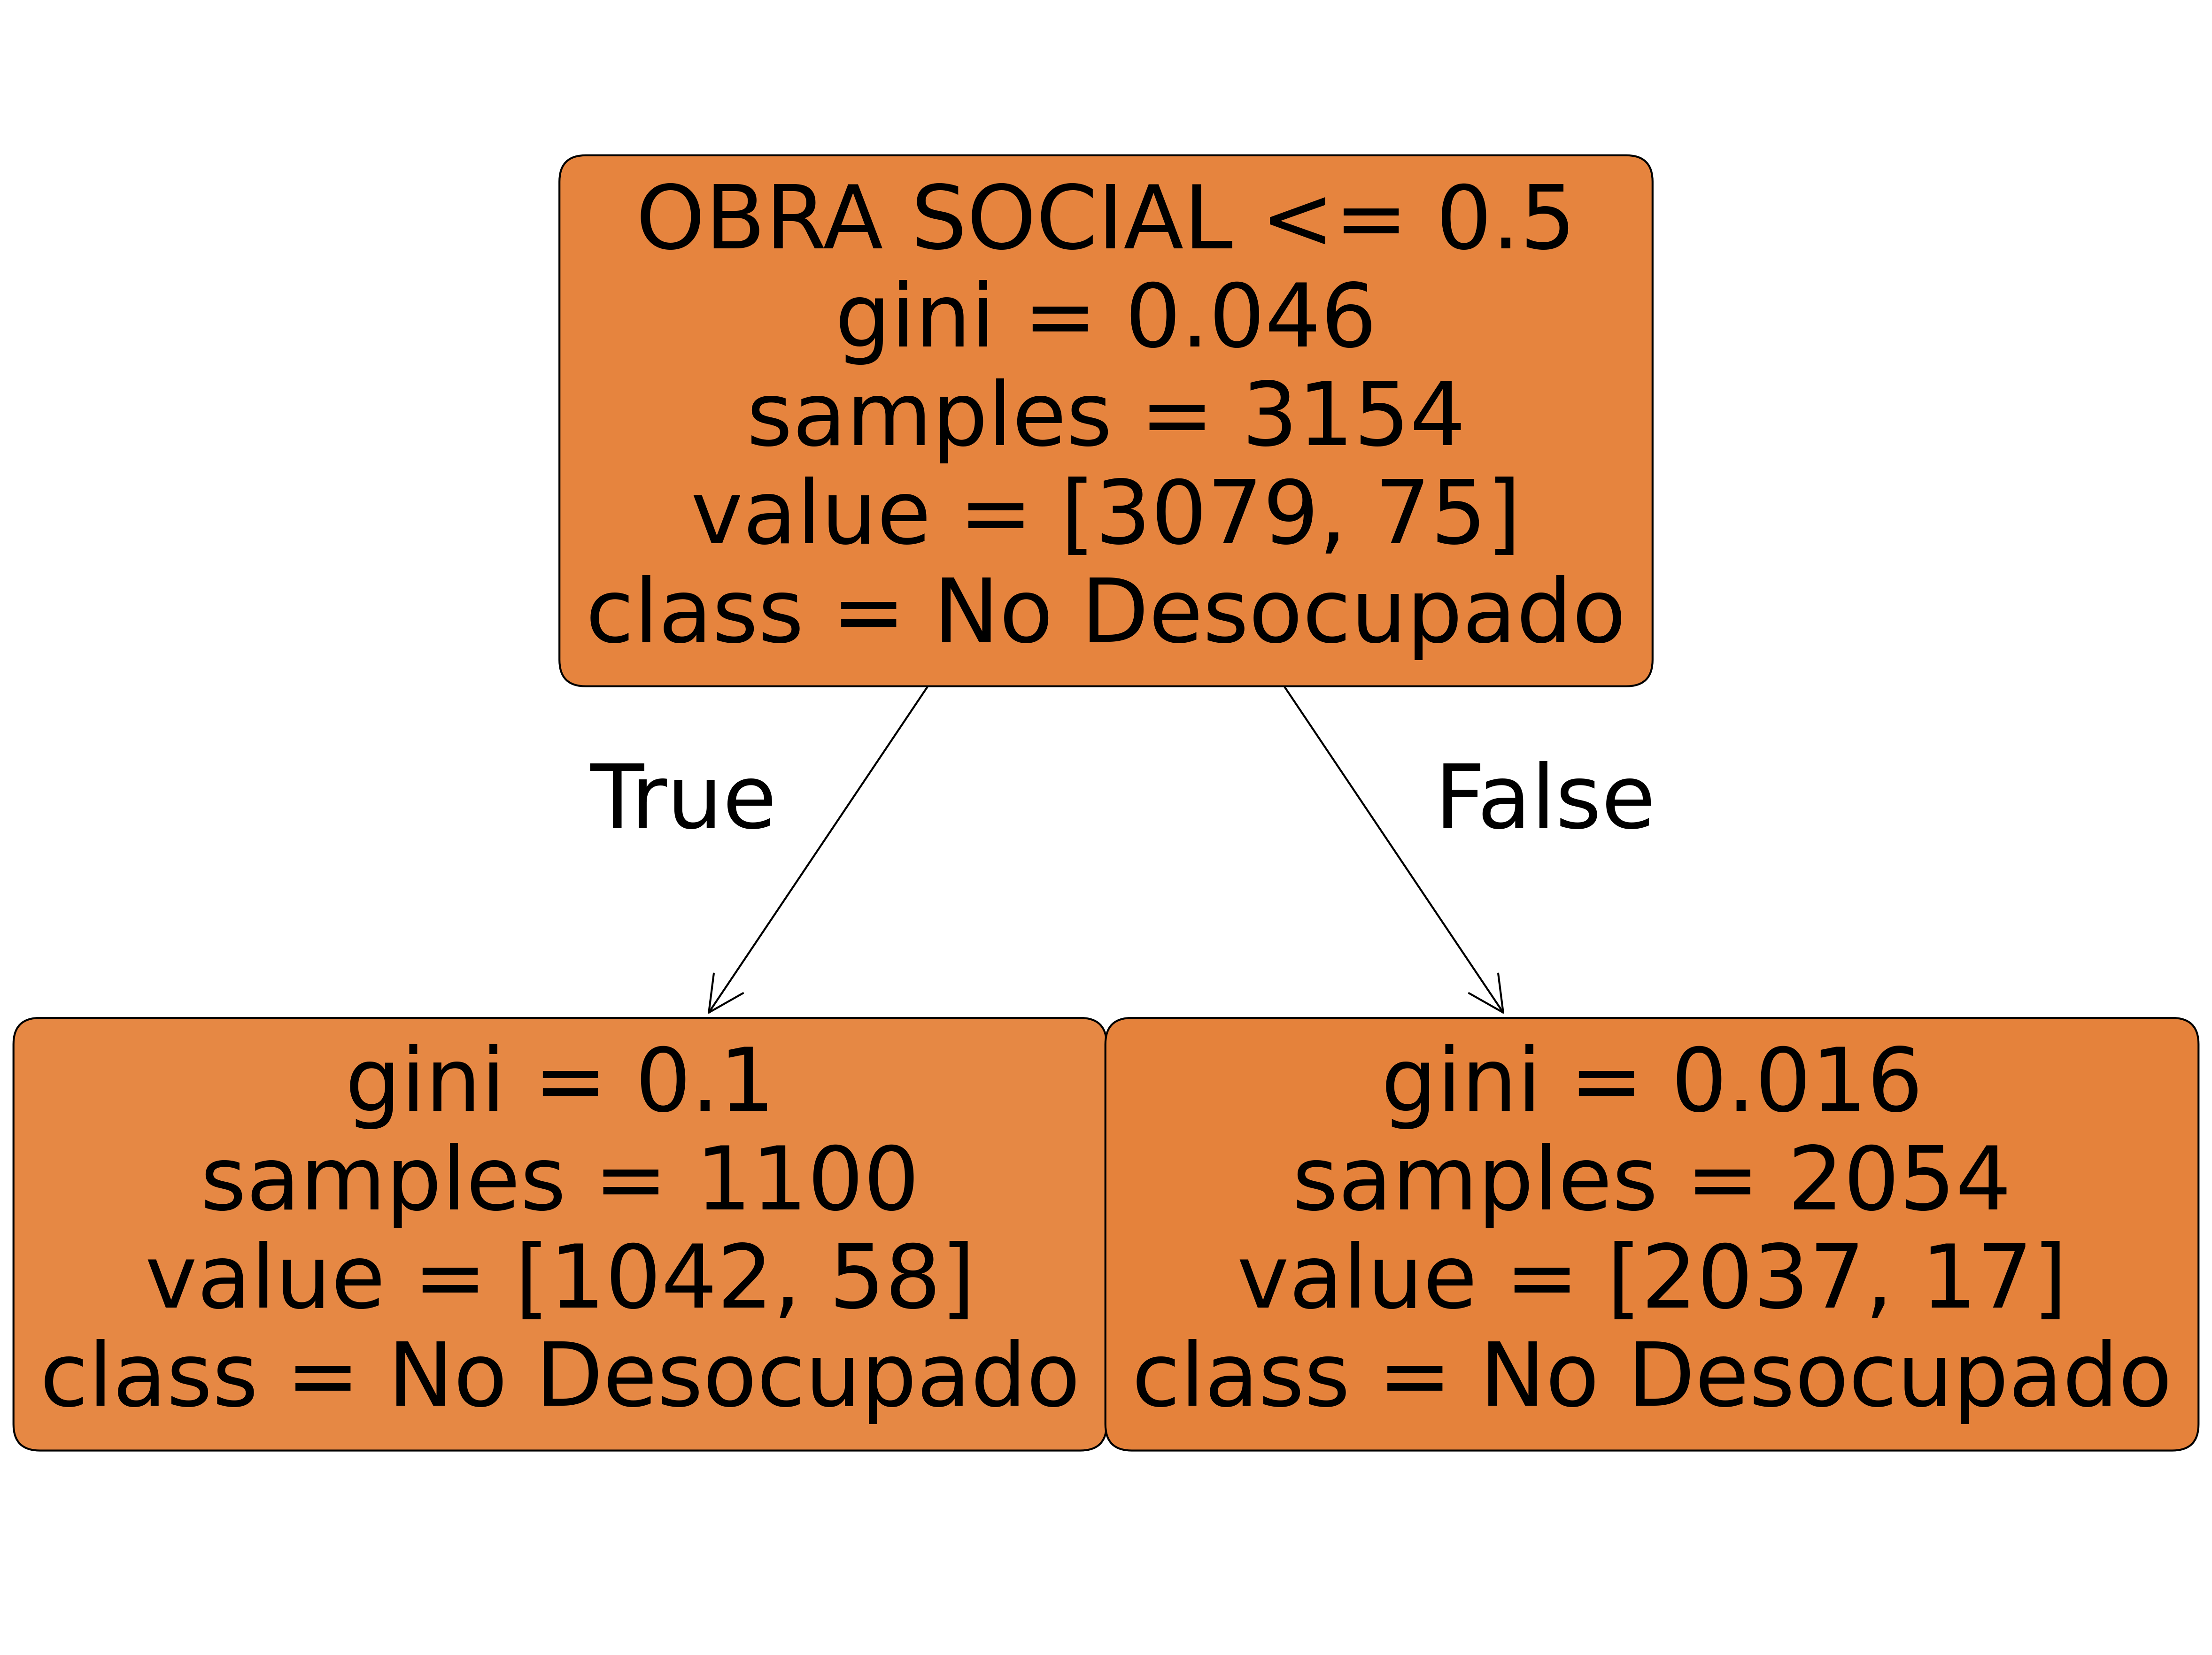
\includegraphics[width=0.45\linewidth]{arbol-2024.png}
\end{figure}

\subsection*{Ejercicio 8}

La Figura~\ref{fig:importancia} muestra los gráficos de importancia de predictores para 2004 y 2024. En ambos casos, el último coeficiente (que tiene importancia 0) es la constante, lo que es consistente con la variable que LASSO descartó.

\begin{figure}[H]
    \centering
    \caption{Importancia de predictores (2004 vs 2024)}
    \label{fig:importancia}
    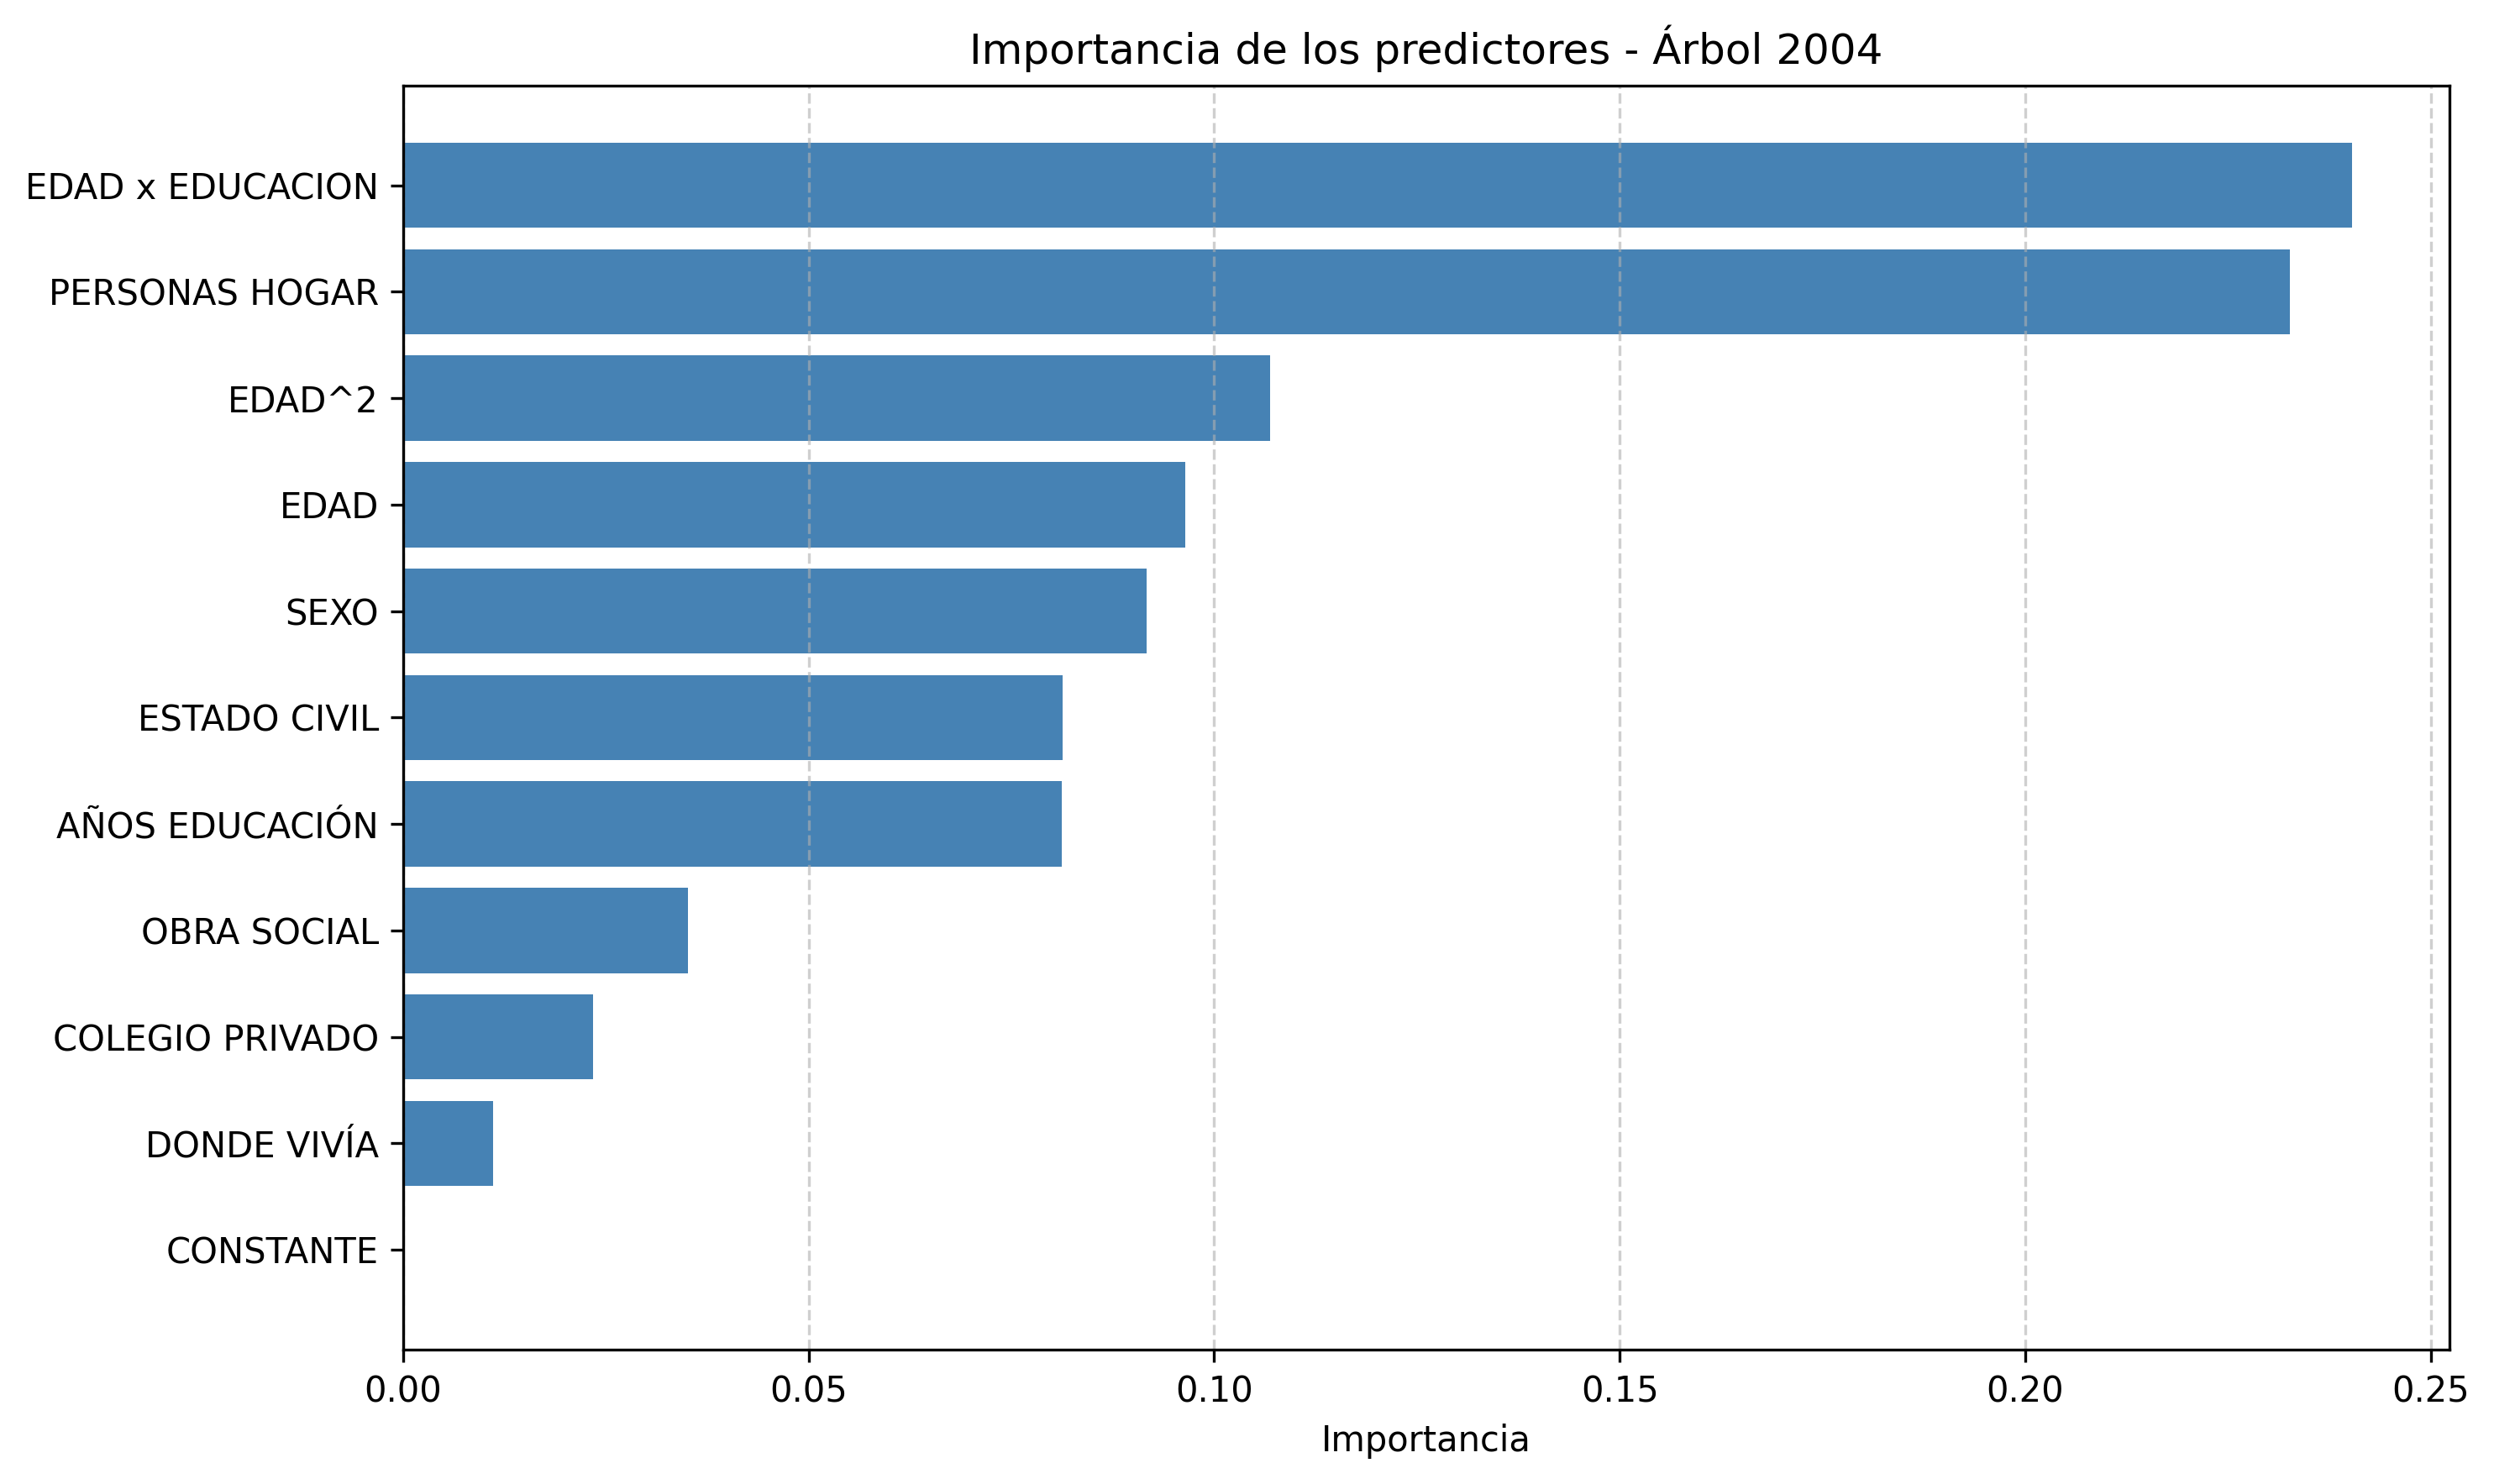
\includegraphics[width=0.45\linewidth]{importancia-2004.png}
    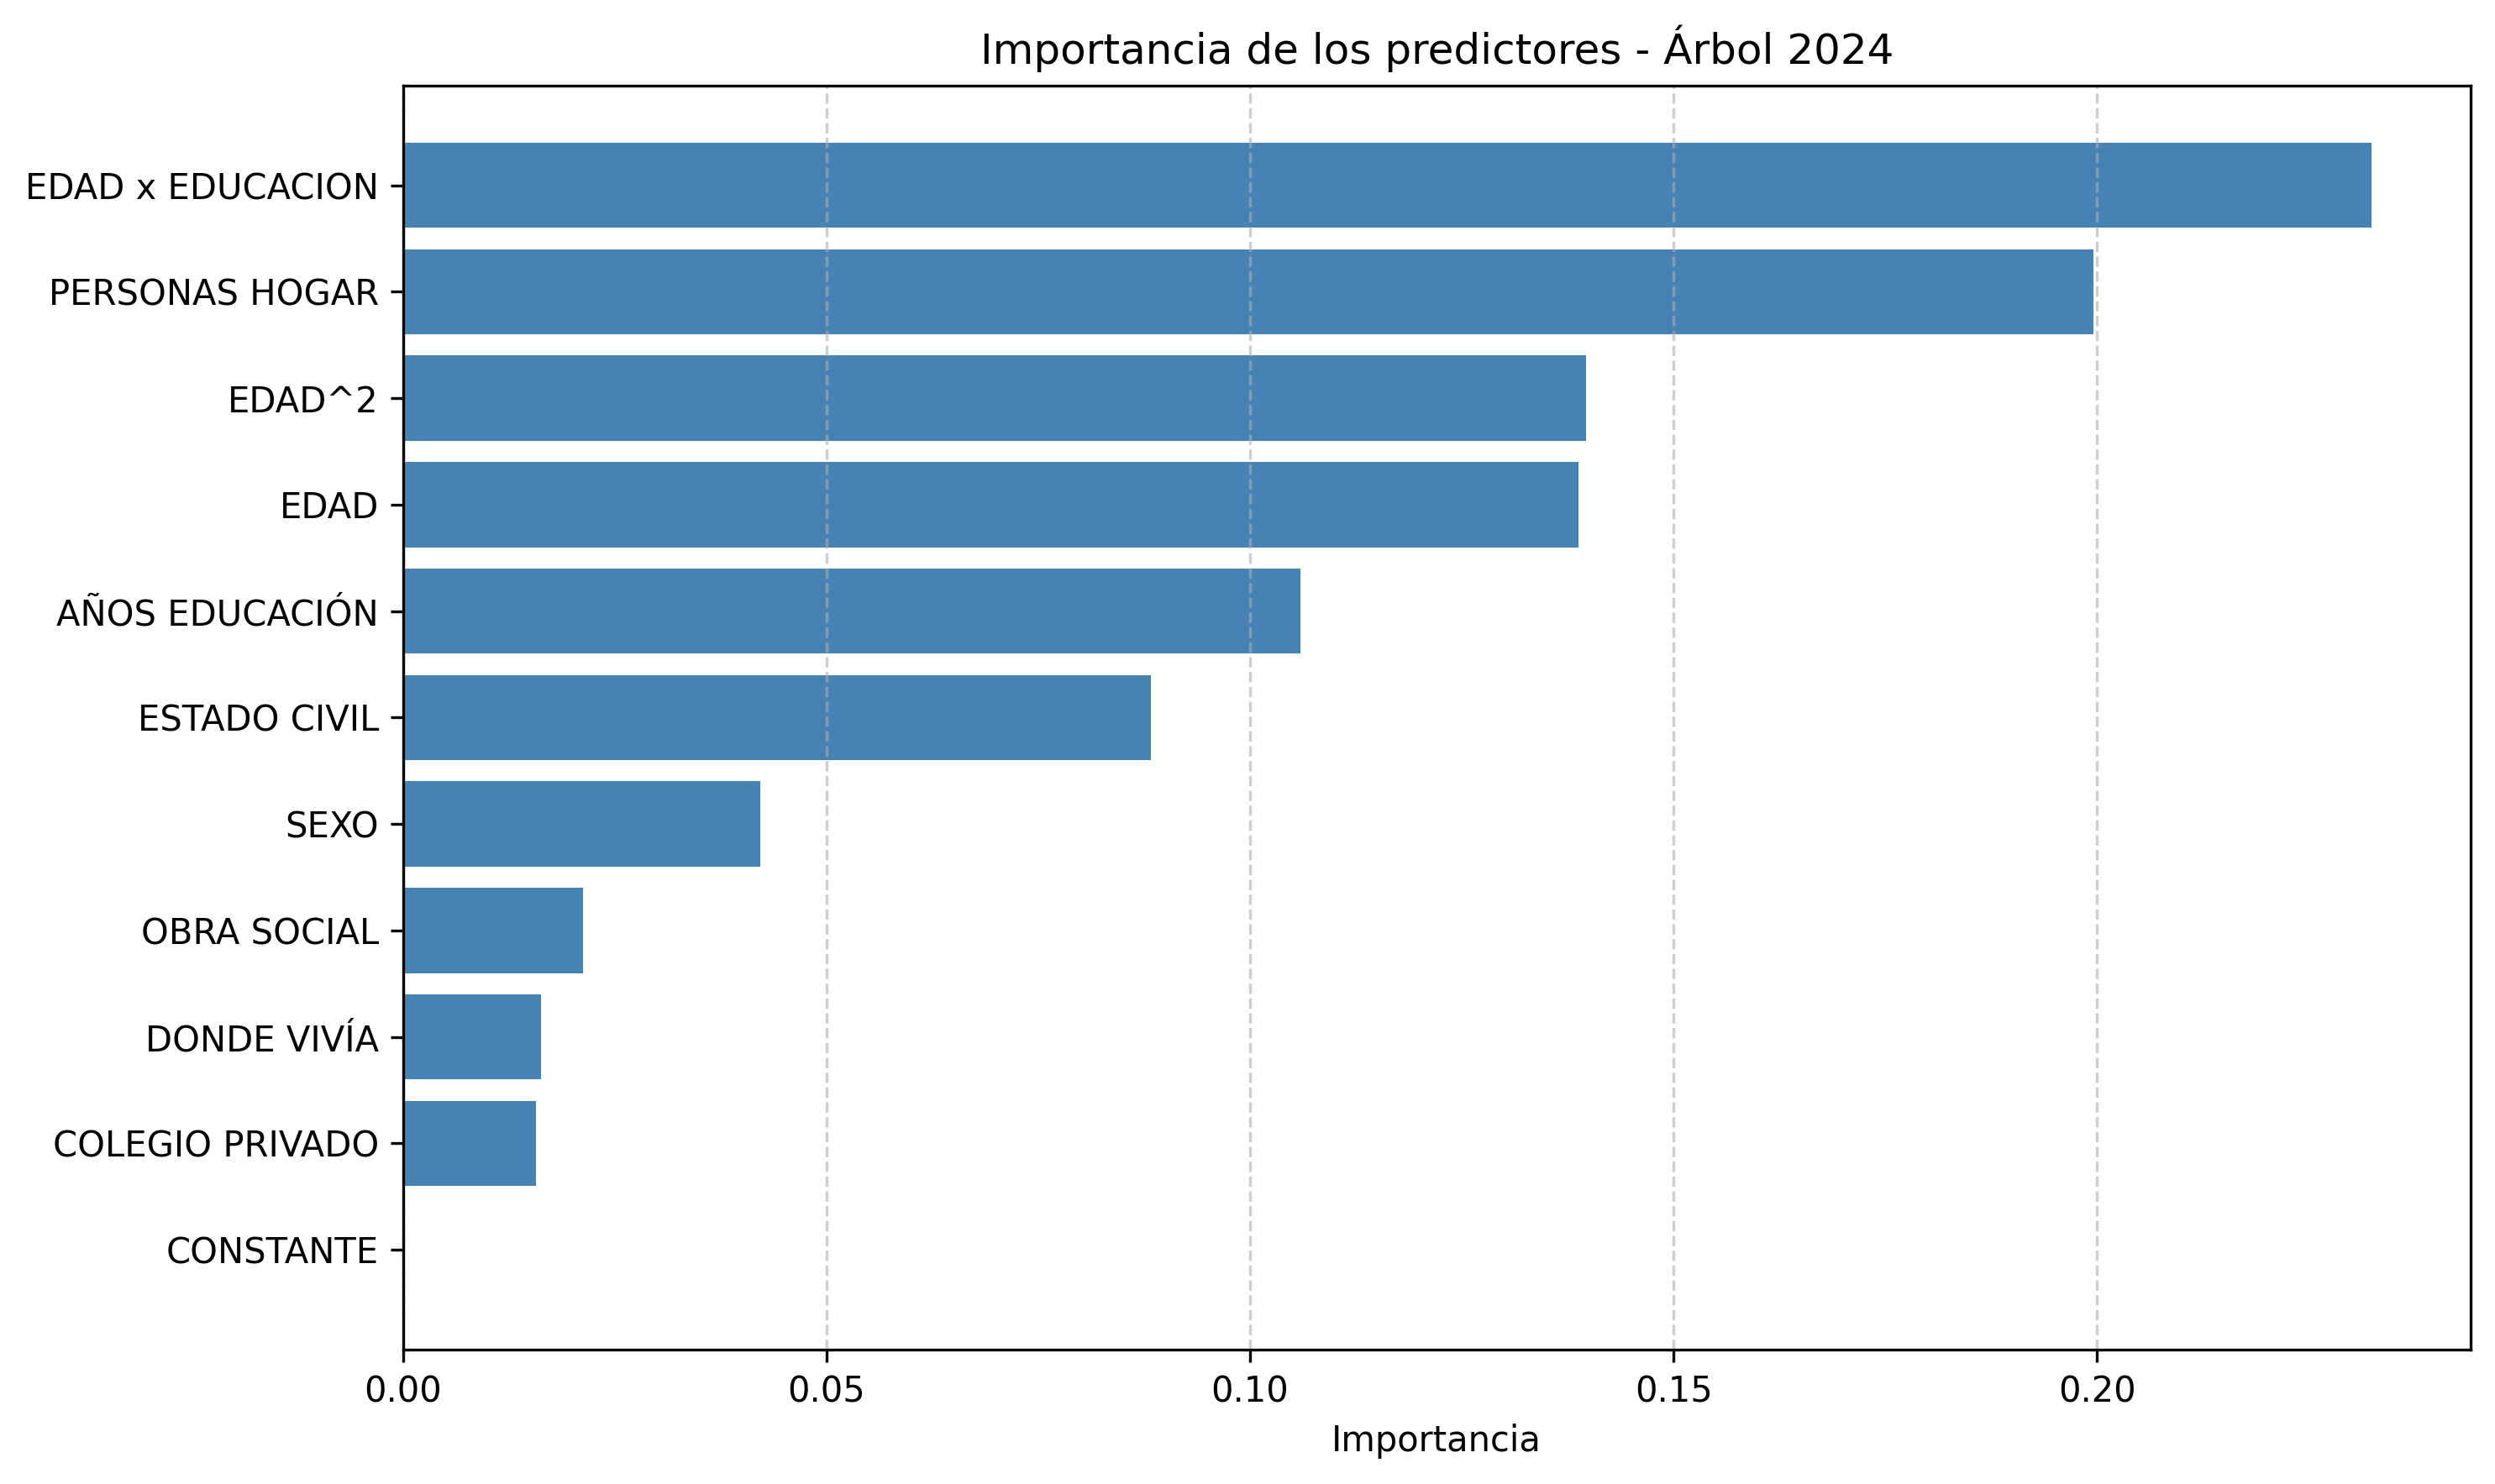
\includegraphics[width=0.45\linewidth]{importancia-2024.png}
\end{figure}

\subsection*{Ejercicio 9}

Los árboles de decisión estimados para 2004 y 2024 muestran un desempeño que parecería ser bueno en \textit{accuracy}, con valores de 95.44\% y 98.15\%, respectivamente. Esto en realidad se debe a que en ambas muestras hay muy pocos desocupados. Asimismo, los errores cuadráticos medios de testeo son bajos: 0.05 para 2004 y 0.02 para 2024, lo que sugiere una buena capacidad general de ajuste. No obstante, al analizar otras métricas más sensibles a clases desbalanceadas, como el área bajo la curva ROC, se observan limitaciones importantes: 0.67 en 2004 y 0.60 en 2024. Las curvas ROC correspondientes se presentan en la Figura~\ref{fig:rocarboles}.

Estas cifras reflejan lo que se observa en las matrices de confusión (Cuadro~\ref{tab:cmarboles}): los árboles nunca predicen la clase desocupado. Aunque se ajustan bien a la mayoría de los casos, están completamente sesgados hacia la clase dominante (no desocupado). Esto implica que, a pesar de su simplicidad, estos modelos fallan en capturar correctamente la minoría, lo cual es especialmente problemático en aplicaciones como el análisis del desempleo, donde identificar desocupados es la parte más importante.

Comparando con los modelos LASSO y Ridge, que también presentan un \textit{accuracy} elevado y MSE similares, pero con mejor discriminación de clases (mayor AUC y algo más de sensibilidad en algunos casos), se evidencia un \textit{trade-off} claro entre interpretabilidad y rendimiento predictivo. Los árboles ofrecen una representación comprensible y visualmente accesible del proceso de decisión, lo cual es valioso para comunicar resultados a audiencias no técnicas. Sin embargo, este beneficio viene a costa de una capacidad predictiva más limitada, especialmente cuando se trata de identificar correctamente clases minoritarias.

En este caso, el uso de un modelo no lineal como el árbol de decisión no aporta una ventaja en términos de performance predictiva respecto a los métodos lineales penalizados. De hecho, los modelos LASSO y Ridge, al incorporar regularización, logran un equilibrio más adecuado entre ajuste y generalización, siendo capaces de capturar patrones más relevantes incluso en contextos de fuerte desbalance. Por lo tanto, si bien los árboles son útiles por su transparencia, para fines puramente predictivos como el de este trabajo, los modelos penalizados resultan más eficaces.

\begin{table}[H]
\begin{center}
\caption{Matrices de Confusión}
\label{tab:cmarboles}
\begin{tabular}{l|rr|rr}
\toprule
 & \multicolumn{2}{c|}{2004} & \multicolumn{2}{c}{2024} \\
 & Pred 0 & Pred 1 & Pred 0 & Pred 1 \\
\midrule
Real 0 & 1381 & 0 & 1328 & 0 \\
Real 1 & 66 & 0 & 25 & 0 \\
\bottomrule
\end{tabular}
\end{center}
\end{table}

\begin{figure}[H]
    \centering
    \caption{Curvas ROC de los árboles (2004 vs 2024)}
    \label{fig:rocarboles}
    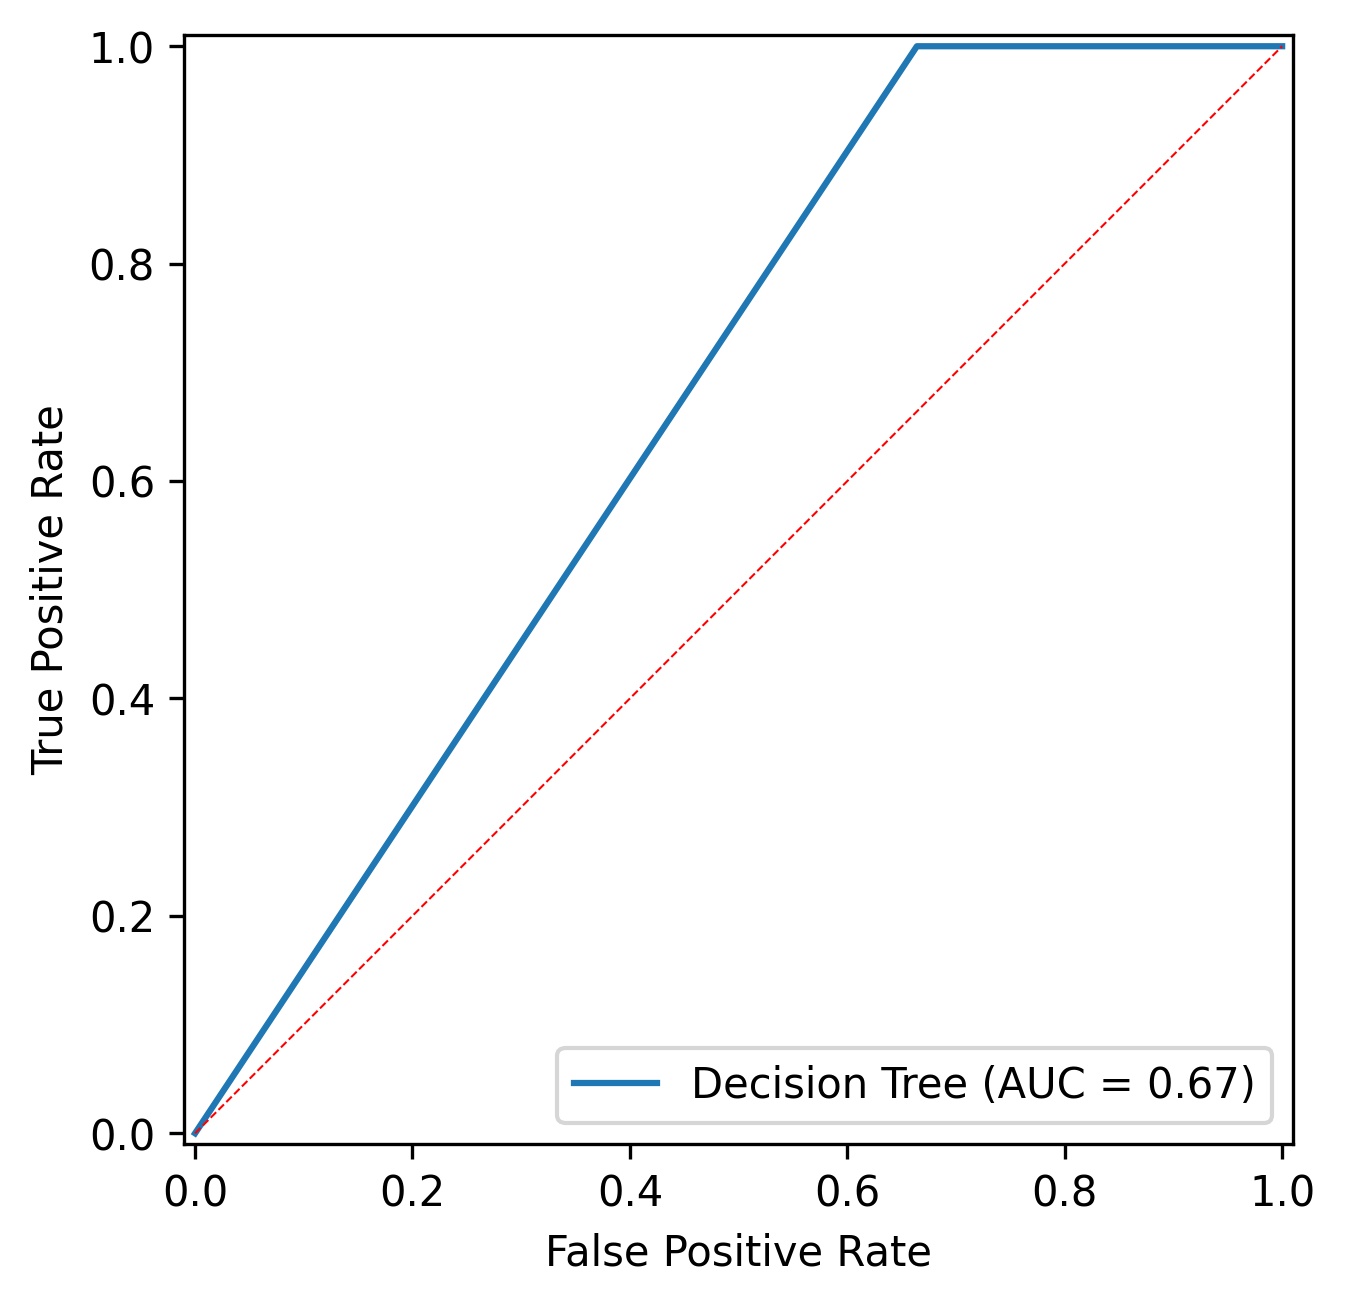
\includegraphics[width=0.4\linewidth]{curva-arbol-2004.png}
    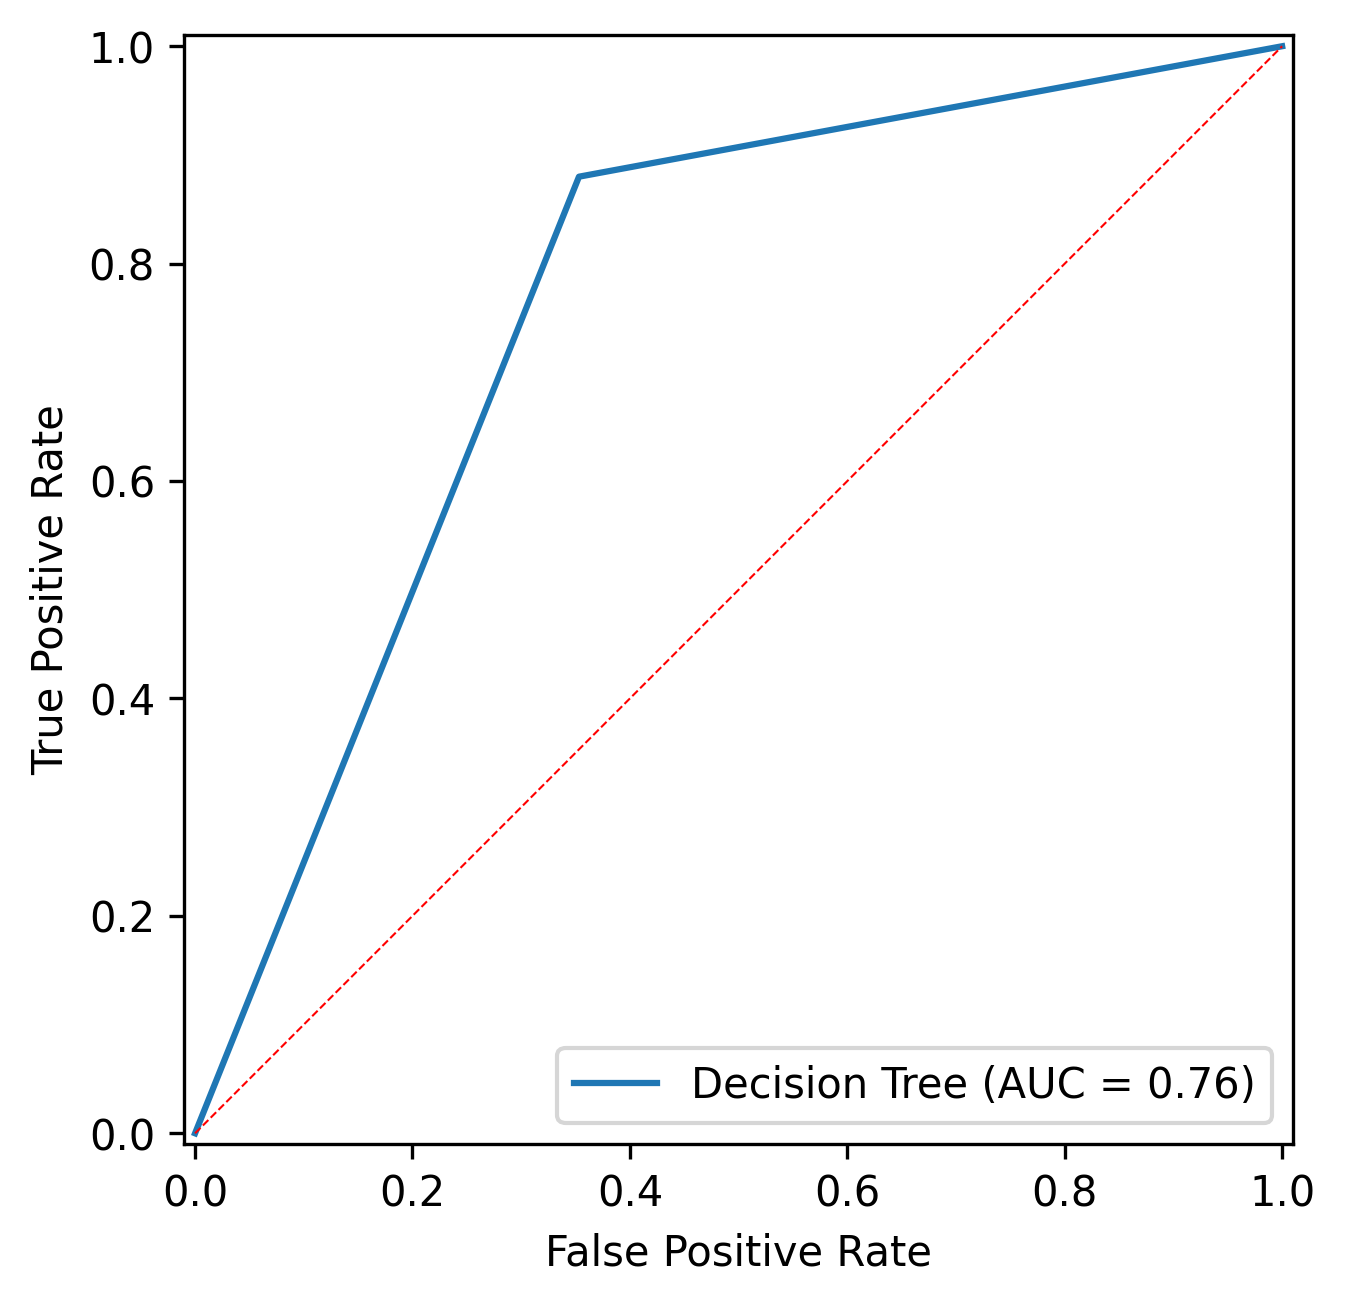
\includegraphics[width=0.4\linewidth]{curva-arbol-2024.png}
\end{figure}

\end{document}
